%% LyX 2.1.4 created this file.  For more info, see http://www.lyx.org/.
%% Do not edit unless you really know what you are doing.
\documentclass[11pt,english,italian,openright]{book}
\usepackage[T1]{fontenc}
\usepackage[latin9]{inputenc}
\usepackage[a4paper]{geometry}
\geometry{verbose,tmargin=3cm,bmargin=3.5cm,lmargin=4cm,rmargin=3cm}
\setcounter{secnumdepth}{3}
\setcounter{tocdepth}{3}
\usepackage{color}
\usepackage{babel}
\usepackage{float}
\usepackage{booktabs}
\usepackage{url}
\usepackage{amsmath}
\usepackage{amssymb}
\usepackage{graphicx}
\usepackage{setspace}
\usepackage{esint}
\onehalfspacing
\usepackage[unicode=true,pdfusetitle,
 bookmarks=true,bookmarksnumbered=false,bookmarksopen=false,
 breaklinks=false,pdfborder={0 0 1},backref=false,colorlinks=false]
 {hyperref}

\makeatletter

%%%%%%%%%%%%%%%%%%%%%%%%%%%%%% LyX specific LaTeX commands.
\providecommand{\LyX}{\texorpdfstring%
  {L\kern-.1667em\lower.25em\hbox{Y}\kern-.125emX\@}
  {LyX}}
\DeclareRobustCommand*{\lyxarrow}{%
\@ifstar
{\leavevmode\,$\triangleleft$\,\allowbreak}
{\leavevmode\,$\triangleright$\,\allowbreak}}
%% Because html converters don't know tabularnewline
\providecommand{\tabularnewline}{\\}
\floatstyle{ruled}
\newfloat{algorithm}{tbp}{loa}[chapter]
\providecommand{\algorithmname}{Algoritmo}
\floatname{algorithm}{\protect\algorithmname}

%%%%%%%%%%%%%%%%%%%%%%%%%%%%%% User specified LaTeX commands.
% pacchetti aggiuntivi
\usepackage{tabularx}
\usepackage{setspace}
\usepackage{amsthm}
\usepackage{rotating}
\usepackage{caption}
\usepackage{epsfig}
\usepackage{indentfirst}
\usepackage{fancyhdr}
\usepackage{url}
\usepackage{cite}
\usepackage[normalem]{ulem}
\usepackage[table]{xcolor}
\usepackage{booktabs}
\usepackage{algpseudocode}

% questa � uno sporca soluzione per gestire il fatto che le versioni
% LTS di Ubuntu/Kubuntu hanno un pacchetto "geometry" vecchio
\include{geometry.sty}

% sistema il numero pagina nelle prime pagine dei capitoli
\fancypagestyle{plain}{
\fancyhead{}
\renewcommand{\headrulewidth}{0pt}
\renewcommand{\footrulewidth}{0pt}
\fancyfoot[OC]{\begin{flushright}\thepage\end{flushright}}
}

% header "carini" per la tesi
\fancyhead{}
\fancyhead[LE]{\slshape \nouppercase \leftmark}
\fancyhead[RO]{\slshape \nouppercase \rightmark}
\fancyfoot[EC]{\begin{flushleft}\thepage\end{flushleft}}
\fancyfoot[OC]{\begin{flushright}\thepage\end{flushright}}
\renewcommand{\headrulewidth}{0.4pt}
\setlength{\headheight}{14pt}

\@ifundefined{showcaptionsetup}{}{%
 \PassOptionsToPackage{caption=false}{subfig}}
\usepackage{subfig}
\makeatother

\usepackage{listings}
\addto\captionsenglish{\renewcommand{\algorithmname}{Algorithm}}
\addto\captionsenglish{\renewcommand{\lstlistingname}{Listing}}
\addto\captionsitalian{\renewcommand{\algorithmname}{Algoritmo}}
\addto\captionsitalian{\renewcommand{\lstlistingname}{Listato}}
\renewcommand{\lstlistingname}{Listato}

%comandi personalizzati
\newcommand{\virgolette}[1]{``#1''}

\begin{document}
\frontmatter
\pagestyle{empty}
\newgeometry{margin=3cm}\begin{titlepage}

\begin{center}
\Large{\textsc{Politecnico di Milano}}\\
\Large{Scuola di Ingegneria Industriale e dell'Informazione}\\
\large{Corso di Laurea Magistrale in Ingegneria Informatica}\\
\large{Dipartimento di Elettronica, Informazione e Bioingegneria}
\par\end{center}

\vspace{0.5cm}


\begin{center}
\begin{figure}[h]
\centering{}\includegraphics[width=0.5\textwidth]{frontespizio/logo-polimi.png}
\end{figure}
\vspace{1cm}

\par\end{center}

\begin{center}
\LARGE{Progettazione dei mashup per dispositivi mobili: un metodo basato sulla modellazione del contesto}\vspace{2cm}

\par\end{center}

\begin{flushleft}
\begin{tabular}{ll}
Relatore:  & Prof.ssa Letizia TANCA\tabularnewline
Correlatori:  & Prof.ssa Maristella MATERA\tabularnewline
	& Prof. Vittorio ZACCARIA
\end{tabular}\vspace{1cm}

\par\end{flushleft}

\begin{flushright}
\begin{tabular}{ll}
Tesi di laurea di: & \tabularnewline
Valerio CASSANI & Matr. 817398\tabularnewline
Stefano GIANELLI & Matr. 817014\tabularnewline
\end{tabular}\vspace{2.2cm}

\par\end{flushright}

\begin{center}
{\large{}Anno Accademico 2014\textendash 2015}
\par\end{center}{\large \par}

\end{titlepage}
\restoregeometry

\cleardoublepage{}

\begin{flushright}
\emph{\selectlanguage{english}%

Too often we forget that genius, too, depends upon the data within its reach, that even Archimedes could not have devised Edison’s inventions 

\bigskip

Ernest Dimnet

\selectlanguage{italian}%
}\cleardoublepage{}
\par\end{flushright}


\chapter*{Ringraziamenti}

\thispagestyle{empty}Vorrei cominciare questa pagina di ringraziamenti con le persone che hanno collaborato a questo progetto.
Un grazie a Letizia e Maristella, che ci hanno sempre seguito in questi mesi in questo lavoro, sostenendoci e aiutandoci in particolare nella parte metodologica. Grazie a Vittorio e Riccardo che ci hanno aiutato nella parte tecnica, facendomi scoprire nuove tecnologie e metodi.
Un ringraziamento particolare va a Stefano che ho conosciuto quando sono entrato in questo team ed è stato un piacere lavorare con lui e penso di aver imparato moltissimo. 
Poi vorrei ringraziare tutte le persone che ho incontrato qui al Politecnico, penso che ognuno mi abbia trasmesso un insegnamento, un modo di lavorare e ho conosciuto dei veri amici disponibili in tutto e per tutto, anche per studiare insieme per gli esami e svolgere i progetti.
Vorrei ringraziare la mia famiglia: i miei genitori, che mi hanno sostenuto anche in questi anni di università, i miei due fratelli, i nonni, zii e tutti gli altri parenti che mi hanno trasmesso una serie di valori che mi porterò per tutta la vita. 

Un grazie particolare va a Rebecca che mi ha sopportato anche nel periodo da tesista, non facendo mai mancare il suo aiuto per qualsiasi cosa avessi bisogno. (PS: prima o poi informatica te la farò passare!)

Per ultimi ma non per importanza vorrei ringraziare la mia compagnia di amici, che sono sempre presenti se era necessario qualche consiglio e per tutte le serate e i momenti che abbiamo trascorso insieme.

\vspace{1cm}

\begin{flushright}
	Valerio
\end{flushright}


\cleardoublepage

Il mio primo ringraziamento va a tutto il gruppo di lavoro che mi ha accolto con tanto affetto e mi ha accompagnato durante tutto il lavoro. Ringrazio Letizia e Maristella per avermi dato la possibilità di lavorare su questo progetto e per essere state sempre disponibili e di estremo aiuto. Ringrazio Vittorio e Riccardo per i preziosi consigli e per avermi spronato a fare sempre di meglio. 

Ringrazio i miei genitori, senza i quali non avrei mai potuto completare questo percorso.

Ringrazio anche il mio fidato compagno di tesi Valerio, capitato per caso ma col quale è stato veramente un piacere condividere questa esperienza. Se questa tesi sarà un successo è anche merito tuo!

Più di un ringraziamento è d’obbligo ad Alessandro, Andrea e Francesca che mi hanno accompagnato in questa avventura. Senza il vostro supporto non sarei mai arrivato a questo giorno! In realtà Andrea dovrei ringraziarti più per le abbuffate, i caffè e i viaggi folli di questi anni.

Devo più di un ringraziamento a Sara. Ci siamo incontrati tardi ma in te ho trovato una vera amica. Le giornate passate assieme al Poli mi mancano molto!

Devo ringraziare il mio fidato amico Andrea, col quale condivido ormai da una vita qualsiasi cosa. Probabilmente non te lo dico spesso ma la tua amicizia significa molto per me, avere il tuo supporto mi ha aiutato molto in questi anni.

Ringrazio Lorenzo, Giacomo, Lorenzo, Nicolò, Elisa, Wanda e Mara, fidati compagni di uscite e vacanze. Con alcuni di voi è stato anche un immenso piacere condividere i meravigliosi anni delle scuole superiori. Sono felice di aver conosciuto ognuno di voi e di aver condiviso tantissime meravigliose esperienze.

Ringrazio Nelya, per aver sopportato tutte le mie lamentele (e io le tue). Hai sempre saputo esattamente cosa dire nei momenti più difficili ma è stato sempre un piacere parlare con te, in qualsiasi situazione, mi sei stata di grandissimo aiuto.

\vspace{1cm}

\begin{flushright}
	Stefano
\end{flushright}\cleardoublepage{}


\chapter*{Sommario}

\thispagestyle{empty}Internet sta diventando una fonte sempre più importante per l'acquisizione di informazioni. Cambiano anche i metodi di interazione: in passato Internet veniva consultato maggiormente da PC mentre ai giorni d'oggi si tende ad accederci tramite smartphone o tablet. Questi dispositivi hanno avuto un progresso tecnologico estremamente rapido, diventando sempre più sofisticati. Tutto questo progresso non porta solo benefici: siamo infatti inondati da una enorme quantità di informazioni, che rendono difficoltoso il processo di ricerca di ciò che è realmente utile.

CAMUS si inserisce proprio in questo contesto: vuole sfruttare le potenzialità messe a disposizione dai dispositivi mobili per fornire informazioni di reale interesse per chi le deve esplorare. Per fare questo si andrà a sfruttare il \emph{contesto} nel quale si trova l'utente, dove per contesto si intende l'insieme di informazioni sulla situazione nella quale si trova l'utente e il proprio profilo personale, cioè le sue preferenze e interessi. Questi dati raccolti verranno sfruttati per cercare dalle fonti più idonee e per filtrare i risultati che sono effettivamente utili nella situazione corrente.

Un altro importante aspetto riguarda la modalità di presentazione di queste informazioni. Si vuole creare un sistema che dia flessibilità nella creazione delle interfacce grafiche attraverso cui mostrare i dati. Questi schemi verranno sfruttati anche per fornire dei dati aggiuntivi relativi alle informazioni cercate, come mappe, informazioni sul meteo e sui trasporti. Si ritiene che l'utilizzo di queste informazioni di supporto possa migliorare la qualità dei dati forniti e completi in modo ottimale le informazioni di base ottenute grazie al contesto.\cleardoublepage{}


\chapter*{Abstract}

\thispagestyle{empty}\selectlanguage{english}%

\textcolor{red}{translate italian abstract}

\selectlanguage{italian}%
\cleardoublepage{}\pagenumbering{roman}
\setcounter{page}{1}
\pagestyle{fancy}\tableofcontents{}\listoffigures
\listoftables
\listof{algorithm}{Elenco degli algoritmi}
\cleardoublepage{}\mainmatter
\renewcommand{\sectionmark}[1]{\markright{\thesection.\ #1}}
\renewcommand{\chaptermark}[1]{\markboth{\thechapter.\ #1}{}}


\chapter{Introduzione\label{ch:introduzione}}

Negli ultimi anni si è assistito a un'enorme diffusione di Internet e soprattutto di una varietà di dispositivi con i quali è possibile accedervi: mentre agli albori esistevano solamente PC \emph{desktop}, con i quali poter visitare pagine per lo più statiche, al giorno d'oggi sono disponibili dispositivi come \emph{smartphone} e \emph{tablet} che ci permettono di rimanere sempre connessi. Grazie al fatto di essere estremamente portatili e semplici da utilizzare essi sono ormai diventati oggetti indispensabili nella vita quotidiana. Lo scorso anno è avvenuto il sorpasso della quantità di traffico generata da \emph{smartphone} e \emph{tablet} rispetto ai PC (Figura \ref{fig:traffico-tipologia-dispositivo}). L'incremento della velocità delle connessioni e il progresso tecnologico ha fatto sì che sia possibile consultare qualsiasi tipo di informazione su internet, dal semplice testo fino a immagini, video, ecc.

\begin{figure}[ht]
	\centering
	\includegraphics[width=\textwidth]{1-introduzione/Immagini/traffico-dispositivi.png}
	\caption[Traffico generato per tipologia di dispositivo]{Traffico generato per tipologia di dispositivo (fonte: Cisco, 2016)\label{fig:traffico-tipologia-dispositivo}}
\end{figure}

Si è persa anche la tradizione che sia un gestore a pubblicare contenuti in quanto ormai sono direttamente gli utenti a produrre la maggior parte delle informazioni disponibili (Figura \ref{fig:analisi-dati-generati}). Questo fenomeno è stato accentuato con la creazione dei \emph{social network}, che permettono di creare collegamenti tra le persone e dove è possibile condividere qualunque cosa che ognuno trova interessante. Gli utenti vengono così coinvolti nella creazione di contenuti di varia natura. Per esempio possono essere anche di tipo multimediale, grazie alla dotazione di fotocamere ad alta risoluzione nei dispositivi.

\begin{figure}[ht]
	\centering
	\includegraphics[width=\textwidth]{1-introduzione/Immagini/dati-generati-consumer.pdf}
	\caption[Analisi della quantità di dati generati]{Analisi della quantità di dati generati (fonte: IDC, 2014)\label{fig:analisi-dati-generati}}
\end{figure}

Come si può notare in Figura \ref{fig:traffico-categoria-applicazione} il traffico video e audio è in costante aumento. In particolare il traffico di video sovrasta tutti gli altri, anche a causa della maggior dimensioni di questi contenuti. Questo fenomeno è incentivato dalla diffusione di servizi che permettono lo \emph{streaming} dei contenuti multimediali come YouTube\footnote{YouTube: \url{https://www.youtube.com}} o Netflix\footnote{Netflix: \url{https://www.netflix.com}}.

\begin{figure}[ht]
	\centering
	\includegraphics[width=\textwidth]{1-introduzione/Immagini/traffico-categoria.png}
	\caption[Traffico generato per categoria di applicazione]{Traffico generato per categoria di applicazione (fonte: Cisco, 2016)\label{fig:traffico-categoria-applicazione}}
\end{figure}

Internet è diventato una fonte immensa di informazioni, che sono destinate ad aumentare. Un recente trend è relativo ai dispositivi connessi, definito \emph{Internet of Things} (Figura \ref{fig:statistiche-iot}). L'idea è che qualsiasi dispositivo può essere connesso a Internet per generare informazioni, in particolare tutti quelli provvisti di sensori che possono fornire dati sullo stato dell'ambiente nel quale si trovano.

\begin{figure}[ht]
	\centering
	\includegraphics[width=\textwidth]{1-introduzione/Immagini/iot-trend.pdf}
	\caption[Statistiche sull'Internet of Things]{Statistiche sull'Internet of Things (fonte: IDC, 2014)\label{fig:statistiche-iot}}
\end{figure}

%Inizio parte del contesto
Uno dei principali problemi che chiunque lavori coi dati vuole cercare di risolvere è ridurre l'\emph{information noise}, migliorando la precisione delle informazioni da mostrare, in maniera che meglio si adattino ai requisiti.

\upe frequente che le informazioni non vengano acquisite unicamente da una base di dati bensì provengano da più fonti, anche di tipologie diverse tra loro (es.: relazionali, XML, ec..). Basti pensare alla moltitudine di servizi presenti nel web.

Questo aumento della quantità di informazioni, se non propriamente controllato, può provocare un ammasso di dati che genera soltanto confusione piuttosto che fornire elementi utili, riducendo i benefici che invece si potrebbero ricavare da tutte queste informazioni. Tuttavia, distinguere le informazioni rilevanti da quelle che non lo sono è un compito tutt'altro che semplice: alcune informazioni potrebbero essere trattate in maniera differente, anche per lo stesso utente, che in diverse situazioni ha bisogno di informazioni differenti. 

Si parla dunque di sistemi \emph{context aware}, che si occupano dell'\emph{acquisizione} del contesto (per esempio tramite l'utilizzo di determinati sensori), l'\emph{astrazione} e il \emph{riconoscimento} del contesto (per esempio associare un determinato stimolo al contesto) e il \emph{comportamento} adatto alla situazione riconosciuta (per esempio l'esecuzione di un'azione innescata dal contesto) \cite{schmidt2003ubiquitous}. L'utilizzo del \emph{contesto} permette la realizzazione di interfacce grafiche innovative e viene spesso utilizzato nella \emph{computazione ubiqua} e nei \emph{dispositivi indossabili}.

%Resta aperto il problema di come visualizzare le operazioni e come ricercare le info in modo semplice (Fornire interfaccia per permettere agli utenti di cercare le informazioni)

Una volta acquisite le informazioni nasce l'esigenza di definire regole su come mostrarle all'utente finale. Con la diffusione di dispositivi mobili sempre più sofisticati si è resa maggiormente necessaria un'esperienza utente semplice che lo guidi durante le sue attività .

%	parlare di come sia conveniente un meccanismo decori le informazioni testuali con contenuti aggiuntivi, come mappe, foto e altre cose dinamiche}

Per questo motivo ha assunto un ruolo di grande importanza l'esperienza d'uso dell'utente (\emph{User Experience}). Infatti se un'applicazione non è ben formata e non è fruibile in modo semplice dall'utente, il numero di utenti che la utilizzeranno calerà sempre di più. Secondo Gary Illyes di Google \virgolette{circa il $ 61\% $ degli utenti che incontrano problemi con siti e \emph{app} su \emph{smartphone} ne abbandonano l'utilizzo volontariamente}\footnote{Search Engine Land Interview to Gary Illyes of Google: \url{http://searchengineland.com/google-may-add-mobile-user-experience-ranking-algorithm-205382}}. Per evitare questo problema è necessario prestare un'attenzione sempre maggiore a come viene progettato tutto il flusso di navigazione dell'utente e a fornirgli i dati necessari per poter sfruttare al meglio l'applicazione. L'aggiunta di elementi comprensibili in modo intuitivo come mappe e foto porta l'utente a utilizzare altre aree della mente, come quella della memoria fotografica. In questo modo l'utente può facilmente acquisire conoscenza utilizzando diversi dati e diverse tipologie di visualizzazione.

%inizio parte di progetto

\upe proprio per cercare nuovi strumenti in grado di migliorare l'esperienza dell'u\-ten\-te nell'esplorazione delle informazioni che nasce il progetto CAMUS. CAMUS (\emph{Context Aware Mobile mashUpS}) si propone come un \emph{framework} per permettere la realizzazione di \emph{mobile app} che si adattino sia alle preferenze dell'utente sia alla situazione nella quale si trova. L'idea è che l'utilizzo di modelli per definire il contesto e per schematizzare la composizione dell'interfaccia grafica possa portare enormi benefici nell'interazione tra utente e applicazione.

Questo paradigma permette la realizzazione di applicazioni flessibili e personalizzate dove la struttura e i contenuti possono variare in fase di esecuzione in base alle esigenze dell'utente e alla situazione nella quale si trova. Inoltre si vuole sfruttare la multimedialità messa a disposizione dei recenti dispositivi mobili per coinvolgere maggiormente l'utente e semplificargli le attività.

Dalla sigla è possibile intuire le due anime principali che sono alla base del progetto: i \emph{mashup} e il \emph{contesto}.

Per la tematica dei \emph{mashup} viene preso in considerazione l'aspetto di acquisire le informazioni da più fonti di diverso tipo. CAMUS prevede un sistema flessibile che permette di acquisire informazioni da diverse risorse, andando così ad aumentare il potere conoscitivo che si può fornire all'utente. Come detto in precedenza bisogna stare particolarmente attenti all'utilizzo di grosse quantità di dati, in quanto se non opportunamente trattate e filtrate possono generare solamente confusione e risultare così poco fruibili dall'utente. Nasce così l'intuizione di utilizzare il contesto come metodo di selezione dei dati che sono più rilevanti per l'utente. Il contesto mette a disposizione lo stato in cui si trova l'utente, le condizioni dell'ambiente che lo circonda e i suoi interessi personali. Si ritiene che queste preziose informazioni possano essere uno strumento determinante per mettere ordine ai dati e fornire così solo le informazioni che sono interessanti.

Nella tesi si andrà ad affrontare la modellazione della situazione nella quale si trova l'utente. \upe un'attività molto delicata, in quanto esistono una moltitudine di parametri che possono definire una particolare situazione. \upe necessario fare una scelta di quali siano gli indicatori più idonei e quali invece possano essere scartati. L'obiettivo è fornire un modello che permetta di definire in maniera adeguata e \emph{semplice} il contesto in modo da agevolare l'utente e rispettando i principi di \emph{User Experience} precedentemente citati.

Certamente il problema principale riguarda l'organizzazione fisica delle informazioni. Visto che CAMUS non viene limitato ad uno specifico contesto, è necessario prevedere un meccanismo che permetta di adattare la visualizzazione di categorie diverse di informazioni. Come è facilmente intuibile mostrare un elenco di film è ben diverso da mostrare un elenco di ristoranti. Un primo punto da snodare è quindi relativo alla creazione di uno schema flessibile che permetta di descrivere come visualizzare queste informazioni sul dispositivo.

Ma non solo: questo schema deve essere anche in grado di raccogliere informazioni di contorno che permettano di migliorare l'esplorazione di quelle principali. Per esempio, se si sta cercando un ristorante può essere d'aiuto avere a disposizione una galleria di foto del locale con i piatti che offre, una mappa che indichi dove si trova il ristorante o alcune informazioni sul meteo, per decidere se prenotare all'esterno o all'interno. Invece se si sta cercando un film può essere sicuramente d'aiuto avere un trailer da vedere per farsi un'idea del film oppure l'elenco dei cinema che l'hanno in programmazione.

Quelle descritte sono operazioni non sempre alla portata degli utenti, soprattutto per quanto riguarda la modellazione del contesto o la composizione dell'interfaccia grafica. Inoltre, quando il contesto diventa in grado di descrivere diverse realtà, assume anche dimensioni notevoli. Avere troppe scelte a disposizione rende vani gli sforzi per cercare di mettere ordine nei dati, in quanto verrebbe solamente spostato il problema a un altro livello. L'utente non conosce a fondo la struttura dei dati e non è in grado quindi di comporre al meglio un'interfaccia completa dei servizi ausiliari. Per agevolare l'utente in queste situazioni si è deciso di dare importanza alla figura dell'\emph{esperto di settore}. L'esperto di settore è colui che conosce a fondo l'ambito di utilizzo di una \emph{CAMUS app}. Si ritiene che questa sua conoscenza permetta di guidare l'utente nelle sue scelte. Uno dei suoi compiti sarà quello di definire insieme all'utente un profilo, in base alle sue esigenze, in modo che dal contesto possano essere eliminati i rami non necessari. Inoltre si occuperà di comporre delle interfacce funzionali sia per la situazione sia per l'utente. In questo modo è possibile avere una varietà di composizioni adatte ai diversi ambiti di utilizzo che si adattino anche alle preferenze dell'utente e ad altri fattori, come la località.

All'esperto di settore vengono delegati compiti che riguardano maggiormente l'ambito nel quale viene utilizzata l'applicazione. Per questo motivo non è necessario che sia una figura con particolari competenze informatiche. Nel \emph{framework} però saranno necessarie delle fasi più tecniche, per il corretto funzionamento della piattaforma. Queste attività sono relative alle configurazioni del sistema, che necessitano di competenze soprattutto per quanto riguarda il funzionamento dei servizi. Per questo motivo si è scelto di introdurre la figura dell'\emph{amministratore}. I suoi compiti sono quelli di creare lo schema globale del contesto, che verrà utilizzato dagli esperti di settore per creare gli schemi personalizzati, e la descrizione dei servizi che il sistema può usufruire per recuperare le informazioni. Può anche dedicarsi all'introduzione di nuovi componenti utilizzabili nella fase di composizione degli schemi visuali.

\section{Caso di studio: il turismo\label{sec:caso-studio-turismo}}

In questa sezione viene introdotto un caso di studio, che serve per validare il modello proposto per CAMUS. Utilizzare un esempio di applicazione del \emph{framework} a un caso reale può essere un utile indicatore al fine di supportare le scelte effettuate e di osservare se sono presenti alcune lacune nella modellazione.

CAMUS ha come obiettivo quello di essere universale, cioè utilizzabile in ambiti anche molto diversi tra loro. Come caso di studio è stato dunque necessario pensare a un ambito che consentisse di sfruttare al meglio le capacità di adattarsi alle varie situazioni nelle quali si può trovare l'utilizzatore dell'\emph{app}.

\upe stato scelto il caso di studio relativo al settore \emph{turistico}, proprio per via della sua dinamicità. In particolare si è preso in considerazione il caso di un'agenzia di viaggi che deve proporre ai propri clienti dei pacchetti di viaggio.

L'ambito turistico calza a pennello per gli intenti di CAMUS; un viaggio incomincia dalla sua pianificazione: prima di partire, il turista si informa sulla destinazione, quali hotel sono disponibili, con quali mezzi di trasporto è più conveniente raggiungere la destinazione, ecc. In questo frangente CAMUS si propone come \virgolette{suggeritore} di esperienze di viaggio: permette all'utente di non concentrarsi sul \emph{dove} vuole andare, ma sul \emph{cosa} vuole fare. Gli viene data la possibilità di scegliere l'esperienza di viaggio che vuole intraprendere e proporgli così i pacchetti che corrispondono alle sue scelte.

Le potenzialità di CAMUS non terminano una volta che il viaggiatore sceglie la sua meta: l'\emph{app} gli servirà \emph{durante} il viaggio per informarsi sulle attività da svolgere, le escursioni disponibili, i ristoranti nei quali cenare, ecc. Per esempio, se un utente vuole provare un ristorante tipico della zona, gli basterà aprire l'\emph{app} CAMUS e selezionare che è interessato nella ricerca dei ristoranti che propongono dei menù \emph{tipici} del luogo. Gli verrà mostrato un elenco dei ristoranti che si trovano nei suoi paraggi che rispettano i criteri definiti. Inoltre gli verranno fornite indicazioni su come raggiungere il ristorante, sfruttando, se specificato nella richiesta, i mezzi pubblici presenti nella destinazione scelta.

Le due figure principali in questo caso di studio sono due: l'\emph{agente di viaggio} e il \emph{turista}. L'\emph{agente} ha il compito di organizzare tutto il viaggio, gestire quindi le prenotazioni, gli spostamenti principali e i soggiorni per il viaggiatore, mentre il \emph{turista} è colui che fisicamente compie il viaggio, che può essere quindi considerato come l'utente finale.

All'agente vengono inoltre demandati i compiti di personalizzazione dell'\emph{app}: questa fase avviene quando il cliente si presenta nell'agenzia di viaggio. A quest'ultimo vengono prima di tutto fatte alcune domande per conoscere il suo profilo, in modo da adattare le scelte che gli verranno mostrate dall'\emph{app}. In questo modo è possibile evitare che al cliente vengano proposte troppe scelte che non siano di suo interesse. Inoltre vengono fissate alcune opzioni che tendono a non cambiare nel corso del viaggio; per esempio se l'utente viaggia con un animale domestico questa scelta sarà sempre la stessa durante tutto il viaggio e non gli verrà chiesta di nuovo.%\footnote{CAMUS si schiera contro l'abbandono degli animali: \url{http://www.emergenza24.org/salvaunamico/}}

L'ulteriore compito che può svolgere l'agente è quello di personalizzare l'aspetto grafico dell'\emph{app} qualora ritenga che sia necessario. Con CAMUS vengono proposti alcuni \emph{template} predefiniti per ogni categoria e viene lasciata libera scelta all'agente se utilizzarli così come sono o modificarli. Una delle motivazioni nella scelta di modificare l'aspetto riguarda l'aggiunta di alcuni servizi di supporto. Per esempio, se l'agente è consapevole che nel luogo in cui vuole andare il cliente le condizioni meteorologiche sono molto variabili e nella versione predefinita dell'\emph{app} non sono presenti informazioni meteo, può aggiungere questa indicazione in modo da fornire al turista un'informazione in più per gestire al meglio la sua vacanza.

Come si può notare da questo breve esempio, l'utilizzo di CAMUS in un'agenzia viaggi permette di fornire un servizio più coinvolgente ai propri clienti. La realizzazione di \emph{app} personalizzate appositamente per un turista permette di effettuare scelte migliori e di proprio interesse. Inoltre estende la capacità dell'agenzia di fornire un'assistenza al proprio cliente anche durante il viaggio: si può affermare che un'\emph{app} CAMUS assume il ruolo di \emph{assistente di viaggio} e guida il turista durante tutte le fasi della sua esperienza di viaggio.

\section{Struttura della tesi}

Viene ora fornita una panoramica sulla struttura di questa tesi:

\begin{itemize}
	\item 
	Nel Capitolo \ref{ch:nozioni-preliminari}, dopo aver introdotto i modelli che saranno utilizzati nel resto della tesi, si discute la letteratura sull'argomento e le tecnologie impiegate per lo sviluppo del prototipo
	\item 
	Nel Capitolo \ref{ch:metodologia-camus} si entra nei dettagli del progetto CAMUS andando a fornire un contesto più ampio di quello appena descritto e mettendo in risalto gli obiettivi che si vogliono raggiungere. In seguito saranno analizzate nel dettaglio le logiche alla base del \emph{framework}
	\item 
	Nel Capitolo \ref{ch:progettazione-alto-livello} viene introdotta l'architettura della piattaforma. Verrà inoltre fornito uno schema del flusso di esecuzione delle attività ed esposto un caso d'uso reale per chiarire meglio la sequenza delle attività
	\item 
	Nei Capitoli \ref{ch:implementazione-backend} e \ref{ch:implementazione-app} viene analizzata nel dettaglio l'implementazione rispettivamente lato \emph{backend} e \emph{mobile app}. Si analizzano i componenti che formano il sistema e le scelte tecnologiche che hanno portato alla realizzazione del prototipo
	\item 
	Nel Capitolo \ref{ch:performance} si andranno ad analizzare le prestazioni della soluzione implementata, simulando alcuni casi d'uso simili alle condizioni di regime della piattaforma
	\item 
	Nel Capitolo \ref{ch:conclusioni} si discuteranno le conclusioni del lavoro relative al progetto e alcuni spunti per futuri miglioramenti al \emph{framework}
\end{itemize}


\chapter{Nozioni preliminari\label{ch:nozioni-preliminari}}


In questa sezione ...

\section{Context-Awareness\label{sec:context-awareness}}

\textcolor{red}{STEFANO\\Informazioni storiche sulle ricerche relative al contesto} \cite{DBLP:journals/sigmod/BolchiniCQST07} \cite{baldauf2007survey}

\subsection{Context Dimension Model\label{sec:context-dimension-model}}

In questa sezione viene presentato nel dettaglio il \emph{Context Dimension Tree} \cite{DBLP:journals/is/BolchiniQT13}, in quanto � il modello di rappresentazione del contesto che � stato selezionato per l'utilizzo nel progetto CAMUS. Nel \emph{Context Dimension Model} il contesto viene rappresentato come un albero $\mathcal{T} = \textless N, E, r \textgreater $, che descrive i possibili contesti nei quali ci si pu� trovare in una data situazione. \`E formato da una radice \emph{r} e un insieme di nodi \emph{N}, che vengono partizionati nei sottoinsiemi dei \emph{nodi dimensione} $N_D$, colorati di nero, e nei \emph{nodi concetto} $N_C$, colorati di bianco, che rappresentano i valori che possono assumere le dimensioni. La radice \emph{r} � un \emph{nodo concetto}, in quanto rappresenta il contesto pi� generale possibile, che corrisponde dunque all'intero dataset.

\begin{figure}[h]
	\centering
	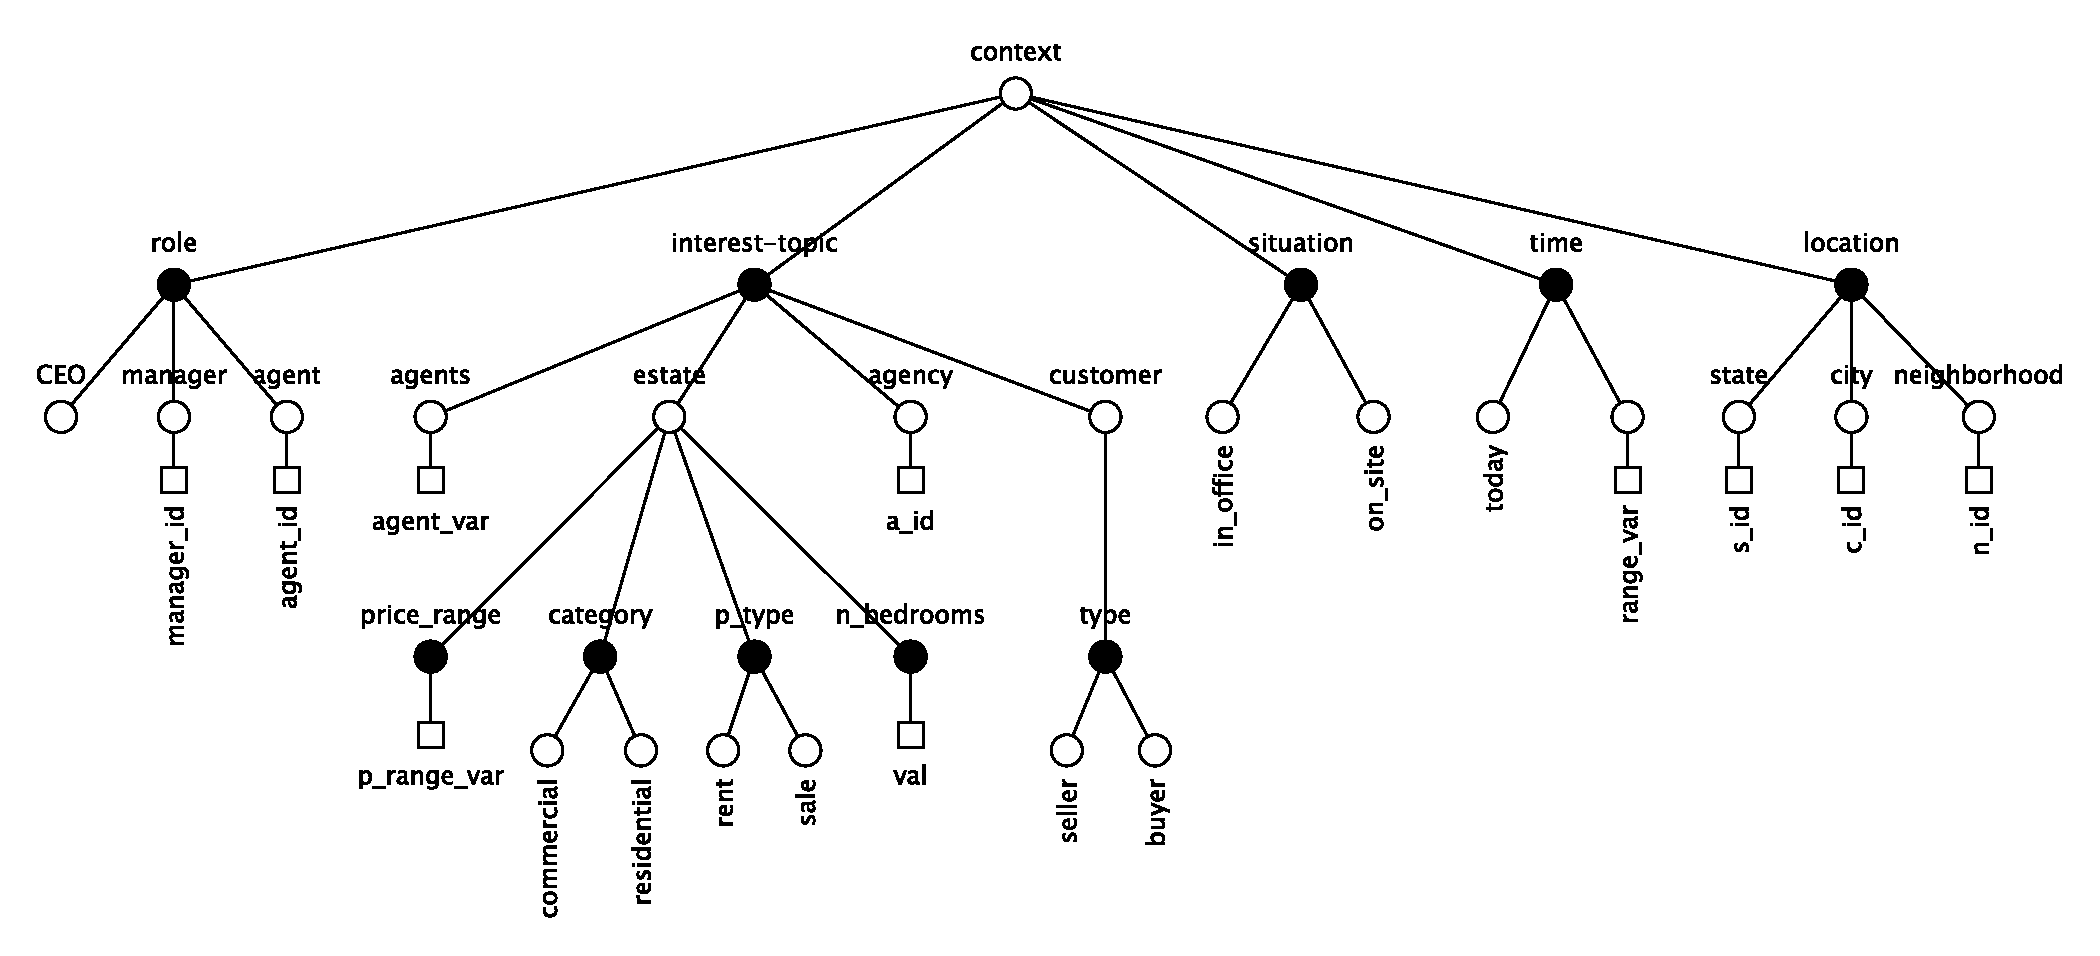
\includegraphics[width=\textwidth]{2-nozioni-preliminari/Immagini/esempio_cdt.png}
	\caption{Context Dimension Tree}\label{fig:context-dimension-tree}
\end{figure}

Le dimensioni che sono dirette discendenti della radice vengono chiamate \emph{dimensioni principali}, perch� definiscono le differenti caratteristiche dell'utente e del contesto nel quale agiscono. Nell'esempio in Figura \ref{fig:context-dimension-tree}, le \emph{dimensioni principali} sono il \emph{ruolo} dell'utente, l'\emph{interfaccia} tramite la quale accede ai dati, l'\emph{interest topic} e la \emph{posizione} in cui si trova. Inoltre, ogni valore pu� essere ulteriormente specializzato tramite \emph{sottodimensioni}, che a loro volta formano un sottoalbero. Per esempio, l'interest topic \virgolette{ordine} pu� essere analizzato in base allo \emph{stato} in cui si trova oppure in base alla sua \emph{tipologia}.

Ogni nodo del CDT � caratterizzato dalla sua tipologia, che pu� essere \emph{dimensione} o \emph{concetto}, e dalla sua etichetta. Ogni nodo pu� essere identificato univocamente tramite l'unico percorso che lo collega fino alla radice. Senza perdita di generalit�, viene adottata l'ipotesi che ogni etichetta sia unica in un albero, quindi ogni nodo pu� essere identificato semplicemente dalla sua etichetta. I collegamenti tra i vari nodi non vengono invece etichettati.

L'alternanza tra nodi \emph{dimensione} e \emph{concetto} fa s� che vengano create delle \emph{generazioni}, ognuna delle quali sar� formata da nodi dello stesso colore, e ogni colore verr� alternato man mano che si prosegue discendendo nell'albero: dunque ogni \emph{nodo dimensione} pu� avere come figli solo nodi di tipo \emph{concetto} e viceversa.

\`E inoltre possibile associare uno o pi� \emph{parametri} ai nodi concetto e ai nodi dimensione che sono foglie dell'albero. Ogni parametro permette di raffinare ulteriormente la selezione dei dati e selezionare un sottoinsieme del dataset particolare. Per esempio, il parametro \virgolette{intervallo} associato al concetto \emph{ordini} permette di indicare un intervallo di date e quindi di selezionare esclusivamente gli ordini che sono riferiti alle date indicate.

Per ogni \emph{nodo dimensione} � possibile selezionare al massimo un nodo concetto tra i suoi figli oppure, se non possiede alcun nodo figlio, deve essere selezionato obbligatoriamente uno ed un solo parametro. L'utilizzo dei parametri aumenta il potere espressivo del modello, in quanto lo rende pi� semplice per l'utilizzo da parte del designer. Si � resa necessaria l'introduzione dei parametri in quanto non tutti i concetti espressi da una dimensione possono essere enumerati. Per esempio, la dimensione \virgolette{costo} pu� assumere infiniti valori ed � quindi pi� appropriato l'utilizzo di un parametro.

Ora che � stato definito il modello � necessario spiegare come viene rappresentato uno specifico \emph{contesto}. Dato un \emph{Context Dimension Tree} $\mathcal{T} = \textless N, E, r \textgreater $, un \emph{contesto} � definito dalla seguente grammatica:

\begin{equation*}
	C =
	\begin{cases}
		\textless context \textgreater \leftarrow \textless context\_element \textgreater\ |\ \textless context\_element \textgreater \land \textless context \textgreater\\
		\textless context\_element \textgreater \leftarrow dim\_name: \textless value\_item \textgreater\ |\ dim\_name\ (\textless parameter \textgreater)\\
		\textless value\_item \textgreater \leftarrow value\ |\ value\ (\textless parameters \textgreater)\\
		\textless parameters \textgreater \leftarrow \textless parameters \textgreater \land \textless parameter \textgreater\ |\ \textless parameter \textgreater\\
		\textless parameter \textgreater \leftarrow param\_name: param\_value
	\end{cases}
\end{equation*}

Un contesto � formato dalla congiunzione tra uno o pi� \emph{elementi del contesto}. Ogni elemento del contesto � formato dal nome della dimensione seguita da uno dei valori scelto tra i nodi che sono suoi figli diretti, oppure dal valore che assume l'unico parametro ad essa associato, nel caso in cui la dimensione � una foglia dell'albero. Ogni valore pu� essere a sua volta raffinato aggiungendo il/i parametro/i ad esso associati. Non � necessario selezionare per forza tutte le dimensioni presenti nell'albero: non selezionare alcun valore relativo ad una dimensione equivale ad essere indifferenti rispetto quella particolare situazione. Ogni dimensione che non viene selezionata non influir� nel processo di acquisizione dei dati contestuali.

Un esempio di contesto �:

\begin{align*}
	C =\ &role : customer\ (\$cid : ``Bill")\ \land \\
		&interest\_topic : orders\ \land \\
		&interface : smartphone
\end{align*}

che rappresenta il contesto in cui il cliente Bill � interessato nel ricevere informazioni sui propri ordini sullo smartphone. Il contesto \emph{C} � quindi composto da tre elementi del contesto.

Infine, dopo aver discusso del modello e di come vengono rappresentati i vari contesti, resta da definire come � possibile acquisire i dati che sono pertinenti ad un determinato contesto. Come evidenziato in \cite{DBLP:journals/cacm/BolchiniCOQRST09}, esistono due strategie principali per definire le associazioni tra i contesti e la porzione di dati rilevanti per i vari contesti, chiamate \emph{configuration-based mapping} e \emph{value-based mapping}.

\begin{figure}[h]
	\centering
	\includegraphics[width=\textwidth]{2-nozioni-preliminari/Immagini/configuration-based-mapping.png}
	\caption{Configuration-based mapping}\label{fig:configuration-based-mapping}
\end{figure}

La strategia \emph{configuration-based mapping} prevede che il designer definisca per ogni contesto possibile la relativa porzione del dataset da mostrare. Questa operazione pu� essere effettuata definendo delle viste nel linguaggio specifico del database adottato. In Figura \ref{fig:configuration-based-mapping} viene mostrato un esempio per il contesto nel quale un manager � interessato alle informazioni relative le sue agenzie. In questo caso il designer specifica delle viste in linguaggio SQL relative al contesto specifico, mettendo in evidenza i dati del personale che lavora nelle agenzie gestite dal manager, i contratti di affitto e vendita ed infine le informazioni relative alle propriet�.

Questa strategia ha il vantaggio di generare delle viste molto precise rispetto al contesto che vogliono rappresentare, ma ha l'enorme svantaggio che deve essere ripetuta per ognuno dei possibili contesti che, com'� facilmente intuibile, possono essere in quantit� molto elevata. Inoltre, se in futuro dovesse essere aggiunta un'ulteriore dimensione, sarebbe necessario modificare le varie associazioni per includere la nuova dimensione.

\begin{figure}[h]
	\centering
	\includegraphics[width=\textwidth]{2-nozioni-preliminari/Immagini/value-based-mapping.png}
	\caption{Value-based mapping}\label{fig:value-based-mapping}
\end{figure}

La strategia \emph{value-based mapping} permette di superare i limiti evidenziati per la strategia precedente. Questa strategia prevede che il designer definisca le viste parziali relative ad un particolare elemento del contesto, indipendentemente dagli altri. Quindi, una volta selezionato un contesto, la vista relativa viene creata da un algoritmo che combina assieme le varie viste parziali definite dai singoli elementi per formare la vista globale adatta allo specifico contesto. La figura \ref{fig:value-based-mapping} mostra come il contesto delll'esempio precedente viene mappato tramite questa strategia. Le linee tratteggiate mostrano le viste parziali che vengono associate ai vari elementi del contesto, mentre nel riquadro in basso viene mostrata la vista globale generata dalla combinazione delle viste parziali. L'algoritmo di composizione delle view parziali � basato sull'utilizzo di diverse policy e operatori di composizione, tra i quali i pi� utilizzati sono \emph{double union}, \emph{double intersection} e \emph{double difference} \cite{DBLP:conf/er/BolchiniQR07}.

\section{I Mashup\label{sec:mashup}}

In questa sezione vengono introdotti i \emph{Mashup}, la seconda anima del sistema CAMUS, e il loro ruolo nell'applicazione finale.
La parola \emph{Mashup}, che significa letteralmente miscuglio o combinazione, � un termine che pu� essere adottato in diversi campi.
Ad esempio, in campo musicale, indicano due o pi� brani le cui tracce audio vengono tagliate e sovrapposte creando un nuovo brano. Un altro esempio � l'ambito dei contenuti video, dove due o pi� filmati o spezzoni sono montati in sequenza per ottenere un video dal significato diverso da quelli originali.
In informatica questo termine assume un significato, perch� i mashup sono applicazioni che utilizzano contenuti provenienti da due o pi� sorgenti, che possono essere servizi privati o pubblici o Web API \cite{DBLP:books/sp/DanielM14}.
Inizialmente la composizione era basata solamente sul contesto del web, perch� permetteva di creare nuove applicazione molto rapidamente, date le API. 

Molto diffuse in questa prima fase sono state le applicazioni basate su Google Maps, come \emph{HousingMaps} \footnote{Housing Maps: \url{http://www.housingmaps.com}}, che si combinava le informazioni tra Google Maps, per quanto riguarda ovviamente le mappe, e Craiglist, un portale che ospita annunci di diversa tipologia (es. lavoro, incontri, ecc...).
Altri esempi sono le mappe interattive che � possibile creare a partire da Google Maps o servizi simili; in questi casi viene arricchita la mappa con altre informazioni, ad esempio traffico, dati demografici o altri dati. 
\begin{figure}[h]
	\centering
	\includegraphics[width=\textwidth]{2-nozioni-preliminari/Immagini/potholes_service.jpg}
	\caption{Potholes Service}\label{fig:potholes}
\end{figure}

L'esempio in Figura \ref{fig:potholes} � un simpatico esempio di mashup che posiziona nella mappa le buche stradali segnalate dagli utenti presenti a Montreal in Canada, fornendo anche la possibilit� di calcolare un itinerario per evitarle o almeno trovarne il meno possibile \footnote{Articolo con altri esempi: \url{http://www.pcworld.com/article/252243/top_10_cool_and_useful_google_maps_mashups.html}}. 

Con lo sviluppo dei social network e delle piattaforme di condivisione di contenuti multimediali, hanno assunto grande importanza i mashup perch� � stato possibile creare nuove applicazioni utilizzando i metadati associati ai contenuti, arricchendo di informazioni il contenuto originale.
La diffusione dei mashup � presente anche in domini pi� critici, soprattutto per la facilit� di creazione e la possibilit� di essere utilizzati anche da utenti non esperti in ambito IT; un esempio possono essere gli \emph{enterprise mashups} \cite{Jhingran:2006:EIM:1182635.1164128}.
La crescita esponenziale della quantit� di informazioni presente nel web, con i Big Data e il moltiplicarsi dei Web Service, ha portato i mashup ad elemento fondamentale nella creazione delle applicazioni, per la possibilit� di filtrare i dati necessari all'utente finale e quindi rendere la visione di una parte significativa delle informazioni provenienti da pi� servizi.
\textcolor{red}{Aggiungere classificazione dei mashups}
Tra le diverse tipologie di mashups elencate in \cite{picozziTesiDottorato}, per quanto riguarda il progetto CAMUS, ci si soffermer� principalmente sui \emph{mobile mashups}.

\subsection{Mobile Mashup\label{sec:mobile-mashup}}

\textcolor{red}{VALERIO\\Informazioni generali sui mashup (non solo mobile)\\
Modello Visuale utilizzato\\
Sottosezione relativa a React Native (spiegare profonda integrazione con la piattaforma di riferimento e confronto con le webview)} \\


I mobile mashups sono l'applicazione dei mashup web ai mobile devices, pensati come applicazioni native che integrano dati provenienti da servizi differenti \cite{Cappiello2013}. 
In CAMUS � stato adottato l'esempio in \cite{Cappiello:2015:UAE:2788341.2735632}, che pone al centro l'interfaccia utente per integrare i dati, dove durante la creazione delle view dell'applicazione � possibile vedere quasi istantaneamente il risultato del visual mapping. In questo approccio si sono volute seguire le linee dettate dalla filosofia di Model-Driven Engineering (MDE), che permettono di generalizzare la creazione degli schemi dell'applicazione, e lasciare l'interpretazione nelle differenti piattaforme. Cos� � possibile creare applicazioni \emph{cross platform}, permettendo di supportare la generazione di codice per applicazioni native. 


\section{Web Services\label{sec:web-services}}

Per \emph{Web Service} si intendono tutti quei software che vengono utilizzati per favorire la comunicazione tra diverse macchine. Secondo la definizione formale fornita dal Consorzio W3C \virgolette{un Web Service � un sistema software creato allo scopo di permettere la comunicazione tra macchine attraverso un network. \upe composto da un'interfaccia descritta in un linguaggio interpretabile dalle macchine (WSDL in particolare). [...]} \cite{world2004web}. In questa definizione viene citato l'utilizzo del protocollo SOAP: in realt�, qualche anno pi� tardi, la definizione � stata estesa \cite{w3c2004web}, includendo nell'elenco:

\begin{itemize}
	\item \emph{REST Web Services}, dove l'obiettivo principale � la manipolazione di \emph{risorse} utilizzando operazioni che non necessitano di mantenere uno stato
	\item \emph{Servizi Web Arbitrari}, dove � possibile esporre a piacimento un insieme di operazioni
\end{itemize}

Il motivo principale che ha spinto verso questa scelta � da ricercare nella definizione stessa di \emph{web service}: l'obiettivo principale � quello di permettere lo scambio di informazioni tra macchine, favorendo l'interoperabilit� tra sistemi e linguaggi di programmazione differenti. La maggior parte dei servizi utilizza il protocollo HTTP come livello di trasporto: questa scelta ha l'enorme vantaggio di poter sfruttare lo stesso protocollo gi� utilizzato per le comunicazioni via internet, cos� da ridurre i costi di gestione necessari per la messa in opera di un diverso protocollo. Nel corso del tempo sono nate diverse tipologie di servizi: alcuni, come SOAP, forniscono una struttura standardizzata da seguire per l'implementazione dei servizi compatibili mentre altri, come REST, forniscono delle linee guida sulla metodologia da seguire per l'implementazione del servizio, ma non sono dipendenti da nessuna tecnologia in particolare. La creazione di servizi che adempiono ad uno specifico compito ha favorito un ulteriore aspetto: la composizione. \upe possibile creare dei servizi che ne sfruttano contemporaneamente diversi al fine di realizzare un processo pi� complesso \cite{weerawarana2005web}. Recentemente questo concetto � stato ulteriormente esteso con la realizzazione dei cosiddetti \emph{mashup} \cite{benslimane2008services}, applicazioni web che permettono di combinare assieme informazioni provenienti da diverse fonti dinamicamente, in modo da fornire un'esperienza utente migliore.

Di seguito vengono analizzate alcune tra le tecnologie e paradigmi pi� utilizzati per la creazione di servizi, tra cui SOAP, REST e GraphQL.

\subsection{SOAP}

\upe l'acronimo di \emph{Simple Object Access Protocol}, fornisce un framework per lo scambio di messaggi.  Utilizza come formato di risposta XML e nella maggior parte si appoggia al protocollo HTTP come livello di trasporto. Vengono scambiate delle \emph{buste}, che contengono le informazioni come interrogare il servizio e come sono rappresentate le risposte. L'architettura SOAP viene distinta per tre caratteristiche principali:

\begin{enumerate}
	\item \textbf{Estensibilit�} Le funzionalit� di base possono essere ampliate attraverso l'utilizzo di estensioni
	\item \textbf{Neutralit�} Non dipende da nessun protocollo di comunicazione in particolare. Quello pi� utilizzato � HTTP, ma esistono delle implementazioni per SMTP, TCP, UDP o JMS per citarne alcuni
	\item \textbf{Indipendenza} Pu� essere utilizzato da diversi linguaggi di programmazione
\end{enumerate}

In seguito, SOAP � stato utilizzato come base per altre tecnologie legate ai web services, come il \emph{Web Services Description Language} (WSDL), che � un'interfaccia di descrizione delle funzionalit� fornite dal servizio, e l'\emph{Universal Description Discovery and Integration} (UDDI), che � un registro dove � possibile ricercare i servizi.

\subsection{REST}

\upe � l'acronimo di \emph{REpresentational State Transfer} ed � uno stile architetturale che definisce determinati vincoli di comportamento per i componenti, connettori e dati che compongono un sistema distribuito ipermediale. \emph{REST} � prima di tutto un paradigma: non vengono infatti menzionati n� i dettagli relativi all'implementazione dei componenti n� i protocolli da utilizzare proprio per concentrarsi sul ruolo dei componenti, sulle interazioni con altri componenti e come interpretare le informazioni. Il termine \emph{REpresentational State Transfer} � stato utilizzato per la prima volta nella tesi di dottorato di Roy Fielding \cite{fielding2000architectural}. \emph{REST} viene largamente utilizzato per descrivere i servizi web, in modo tale da non generare contraddizioni durante l'implementazione. I sistemi che rispettano i principi \emph{REST} vengono chiamati \emph{RESTful}. Nella maggior parte dei casi, i sistemi \emph{RESTful} comunicano attraverso i verbi standard del protocollo HTTP (GET, POST, PUT, DELETE, ecc.). Utilizza come interfaccia per comunicare con i sistemi esterni le \emph{web resources}, identificate tramite un \emph{Uniform Resource Identifier} (URI). L'applicazione dei vincoli definiti dall'architettura permette di ottenere i seguenti vantaggi: performance, scalabilit�, semplicit�, manutenibilit�, visibilit�, portabilit� ed affidabilit�.

I vincoli definiti dall'architettura sono:

\begin{itemize}
	\item \textbf{Client-server} C'� una separazione delle attivit� che devono essere eseguite sul client e sul server. Per esempio, i client non devono occuparsi della memorizzazione dei dati, che rimane interna al server, in modo da favorire la \emph{portabilit�} del codice del client. Il server invece non deve preoccuparsi dell'interfaccia utente e dello stato dell'utente, in modo da rendere l'implementazione del server pi� semplice e \emph{scalabile}. Il client e il server possono essere sostituiti e sviluppati separatamente fintanto che le interfacce tra di essi rimangono immutate
	\item \textbf{Stateless} Lo stato non deve essere assolutamente salvato sul server. Ogni richieste che proviene dal client deve contenere tutte le informazioni necessarie alla sua esecuzione. Sar� compito del client mantenere memorizzato lo stato corrente. Lo stato della sessione pu� per� essere trasferito dal server verso un ulteriore servizio di memorizzazione, per esempio un database, per un periodo di tempo limitato. Al client viene affidato il compito di decidere quando � pronto a passare ad un nuovo stato
	\item \textbf{Cacheable} Sia il client sia il server possono effettuare caching delle risposte. Le risposte per� devono essere innanzitutto definire se possono essere salvate in cache o meno, in modo da limitare situazione nelle quali il client utilizza informazioni non corrette o non pi� valide. Implementare un ottimo sistema di cache permette di ridurre il numero di interazioni tra il client e il server, migliorando la scalabilit� e le performance del sistema
	\item \textbf{Layered system} Un client non pu� specificare se � connesso direttamente al server di pi� basso livello oppure ad un server intermediario. L'utilizzo di server intermediari permette di migliorare la scalabilit� del sistema, tramite l'utilizzo di load balancer e di cache distribuite. Possono inoltre fornire ulteriori misure di sicurezza
	\item \textbf{Uniform interface} L'utilizzo delle \emph{uniform interface} permette di semplificare e disaccoppiare i vari componenti dell'architettura, rendendo possibile lo sviluppo indipendente delle varie parti del sistema. I quattro vincoli riguardo le \emph{uniform interface} sono:
	\begin{enumerate}
		\item \textbf{Identificazione delle risorse} Le singole risorse vengono identificate nella richiesta tramite, per esempio, un \emph{URI}. Le risorse sono concettualmente separate dalle rappresentazioni che vengono inviate al client. Per esempio, un server pu� inviare dati dal database come HTML, XML o JSON, che sono diversi dalla rappresentazione interna del server
		\item \textbf{Manipolazione delle risorse tramite le rappresentazioni} Ogni rappresentazione di una risorsa che viene inviata al client deve contenere tutte le informazioni che permettano la modifica o la eliminazione della risorsa
		\item \textbf{Messaggi autoesplicativi} Ogni messaggio deve contenere informazioni riguardo come trattare l'informazione che porta con s�, tramite per esempio i \emph{media type}
		\item \textbf{Sfruttamento dell'hypermedia (HATEOAS)} I client possono effettuare delle azioni che vengono dinamicamente messe a disposizione dal server tramite hypermedia (es.: link). Ad eccezione dello stato iniziale, il client conosce le azioni che possono essere eseguite a partire da una data rappresentazione solamente attraverso le azioni che essa espone
	\end{enumerate}
\end{itemize}

Applicando i principi REST alle API dei servizi web si ottengono quelle che vengono definite \emph{RESTful API}. Le \emph{RESTful API} che sfruttano il protocollo HTTP sono definite tramite le seguenti caratteristiche:

\begin{itemize}
	\item Possiedono un URI di base
	\item Definiscono un media type, che indica il formato della risposta, che nelle implementazioni pi� comuni � JSON
	\item Utilizzano i verbi standard del protocollo HTTP (es.: OPTIONS, GET, PUT, POST e DELETE)
	\item Mettono a disposizione dei link come referenza per passare alle risorse correlate
	\item Utilizzano dei link come referenza dello stato
\end{itemize}

Solitamente ad una URI pu� essere associata una funzione diversa in base al verbo con la quale viene chiamata, come si pu� notare nell'esempio in Tabella \ref{table:esempio-rest-api}.

\begin{table}[h]
	\caption{Esempio RESTful API}
	\label{table:esempio-rest-api}
	\noindent\makebox[\textwidth]{%
	\begin{tabularx}{1.3\textwidth}{lXXXX}
		\toprule
		\thead{Risorsa} & \thead{GET} & \thead{PUT} & \thead{POST} & \thead{DELETE} \\
		\midrule
		\url{http://api.example.com/resources/} & \textbf{Elenca} le URI insieme ad eventuali altri dettagli sulla collezione & \textbf{Sostituisce} la collezione con un'altra & \textbf{Aggiunge} un nuovo elemento alla collezione. L'URI viene generato automaticamente e restituito dall'operazione & \textbf{Elimina} l'intera collezione \\
		\hline
		\url{http://api.example.com/resources/item17} & \textbf{Restituisce} una rappresentazione dell'oggetto, espresso con un particolare \emph{media type} & \textbf{Sostituisce} l'elemento della collezione o, se non esiste, ne crea uno nuovo & \textbf{Crea} un nuovo elemento & \textbf{Rimuove} l'elemento dalla collezione \\
		\bottomrule
	\end{tabularx}}
\end{table}

\subsection{GraphQL}

\emph{GraphQL} �, come suggeriscono le ultime due lettere del nome, un \emph{query language}, creato come supporto alla realizzazione di applicazioni client, che mette a disposizione una sintassi intuitiva e flessibile ed un sistema che permette al client di specificare i requisiti e le interazioni sui dati \cite{website:graphql-specs}. Rispetto all'approccio REST, \emph{GraphQL} permette di effettuare richieste pi� efficienti dei dati ed evita la duplicazione della logica lato server che pu� verificarsi nel caso di endpoint personalizzati. Una delle principali differenze rispetto a REST riguarda la possibilit� di lasciare al client la scelta dei dati da ricevere. Questa modifica nasce dall'idea che � il client a conoscere nel dettaglio quali dati servono per comporre la view e quindi gli viene delegata la responsabilit� di richiedere solo quelli essenziali all'interno della query.

Alla base di \emph{GraphQL} ci sono i seguenti principi:

\begin{itemize}
	\item \textbf{Gerarchico} Una buona parte dei prodotti sviluppati implica la creazione e manipolazione di view gerarchiche. Per mantenere coerenza con la struttura delle applicazioni, le query \emph{GraphQL} sono esse stesse strutturate gerarchicamente. La query viene plasmata esattamente come i dati che deve restituire. \upe un metodo naturale per permettere ai client di descrivere i vincoli sui dati
	\item \textbf{Basato sul prodotto} \emph{GraphQL} � stato creato tenendo ben presenti i requisiti delle view e del come gli sviluppatori di front-end li esplicitano.
	\item \textbf{Tipizzato} Ogni server \emph{GraphQL} definisce il proprio schema specifico per l'applicazione in uso. Le query vengono eseguite a partire dal contesto definito da questo schema. Inoltre vengono effettuati dei controlli al fine di verificare che la query sia sintatticamente corretta e valida  prima di essere eseguita
	\item \textbf{Query definite dal client} Negli schemi viene inoltre definito il formato della risposta, compresa la tipologia di ogni dato. Sar� poi il client a specificare esattamente quali sono le informazioni che gli interessano. Rispetto ad altri approcci, dove � il server a decidere quali dati restituire ai client, in \emph{GraphQL} invece vengono restituiti solamente i dati che vengono richiesti e nulla di pi�
	\item \textbf{Introspettivo} Qualsiasi schema \emph{GraphQL} pu� essere interrogato tramite query. In questo modo � possibile conoscere la struttura globale dello schema, cos� come le query che sono permesse e quali dati possono essere richiesti. Queste introspezioni servono come base per vari tool per avere una visione completa dello schema che viene esposto dal server
\end{itemize}

\begin{center}
	\begin{minipage}[t]{0.5\textwidth}
		\begin{lstlisting}[caption=Esempio di query GraphQL, label=lst:esempio-query-graphql]
{
	!user!(@id@: ~2~) {
		!name!
		!surname!
	}
}
		\end{lstlisting}
	\end{minipage}%
	\hspace{5mm}%
	\begin{minipage}[t]{0.4\textwidth}
		\begin{lstlisting}[caption=Esempio di risposta, label=lst:esempio-risposta-graphql, style=json]
{
	"user": {
		"name": "Mario",
		"surname": "Rossi"
	}
}
		\end{lstlisting}
	\end{minipage}	
\end{center}

Nel Blocco \ref{lst:esempio-query-graphql} viene riportato un semplice esempio di query scritta tramite \emph{GraphQL}. Con questa query si vogliono acquisire i dati relativi all'utente con identificativo 2, ed in particolare si � interessati a ricevere il suo \emph{nome} e \emph{cognome}. Nel Blocco \ref{lst:esempio-risposta-graphql} viene invece mostrato un esempio di risposta che viene ricevuta dalla server.

\emph{GraphQL} fornisce inoltre un'altra funzionalit� estremamente utile: le \emph{connessioni}. Una \emph{connessione} permette ad un oggetto di definire i legami che ha con altri oggetti, anche di tipo diverso dal suo. In questo modo � possibile richiedere direttamente le informazioni riguardo altri oggetti tramite un'unica query; questa caratteristica non � presente nei sistemi REST e permette di ottenere un netto miglioramento delle performance. Inoltre, GraphQL mette a disposizione per ogni connessione la \emph{paginazione} dei risultati, ossia la possibilit� di richiedere un determinato numero di elementi ad ogni richiesta. Ad ogni oggetto viene automaticamente associato un \emph{token} che lo identifica univocamente: in questo modo � possibile chiedere ulteriori elementi in una seconda query, specificando il \emph{token} dell'oggetto di partenza.

\begin{center}
	\hspace*{-1.5cm}
	\begin{minipage}[t]{0.63\textwidth}
		\begin{lstlisting}[caption=Esempio di connessione GraphQL, label=lst:esempio-connessione-graphql]
{
	!user! (@id@: ~4802170~) {
		!id!
		!name!
		!isViewerFriend!
		!profilePicture! (@size@: ~50~) {
			!uri!
			!width!
			!height!
		}
		!friendConnection!(@first@: ~2~) {
			!totalCount!
			!friends!: {
				!id!
				!name!
			}
		}
	}
}
		\end{lstlisting}
	\end{minipage}%
	\begin{minipage}[t]{0.63\textwidth}
		\begin{lstlisting}[caption=Esempio di risposta, label=lst:esempio-risposta-connessione-graphql,style=json]
{
	"user": {
		"id": 4802170,
		"name": "Lee Byron",
		"isViewerFriend": true,
		"profilePicture": {
			"uri": "cdn://pic/4802170/50",
			"width": 50,
			"height": 50
		},
		"friendConnection": {
			"totalCount": 13,
			"friends": [
				{
					"id": 305249,
					"name": "Stephen Schwink"
				},
				{
					"id": 3108935,
					"name": "Nathaniel Roman"
				}
			]
		}
	}
}
		\end{lstlisting}
	\end{minipage}	
\end{center}

Nel Blocco \ref{lst:esempio-connessione-graphql} viene mostrata una query pi� complessa della precedente. La \emph{connessione} viene definita da \virgolette{friendConnection}, che viene utilizzata per recuperare gli amici dell'utente corrente. Si vuole far notare che gli oggetti che vengono restituiti nel campo \virgolette{friends} sono dello stesso tipo dell'utente richiesto in origine: questo vuol dire che � possibile produrre infiniti livelli gerarchici. Se, all'interno di un utente amico, si specifica di nuovo la connessione \virgolette{friendConnection}, verranno restituiti anche gli amici di quello specifico utente. Altro punto interessante, come citato in precedenza, delle \emph{connessioni} riguarda la possibilit� di richiedere solo un sottoinsieme dei risultati: nell'esempio vengono richiesti solamente i primi due amici dell'utente. Come si pu� notare nel Blocco \ref{lst:esempio-risposta-connessione-graphql}, vengono restituiti solamente i primi due amici, nonostante il campo \virgolette{totalCount} indichi che l'utente ha in totale 13 amici. Tramite ulteriori query possono essere richiesti gli altri amici dell'utente.

\section{Stato dell'arte\label{sec:stato-arte}}

\textcolor{red}{Descrizione dei principali "competitor" (IFTTT, Atooma, Swagger, Appery.io, Kimono, AdAPT, Yahoo Pipes, JackBe Presto, Mashart.org, Peudom)}


\chapter{Il Progetto CAMUS\label{ch:camus}}

In questo capitolo ...

\section{Panoramica del progetto}

\textcolor{red}{Introduzione al progetto\\
	Spiegare le due anime, senza dire il perch�\\
	Dare un'idea di come sono strutturati i vari ambienti (server, web app e app mobile)}

\section{Obiettivi del progetto\label{sec:obiettivi-progetto}}

\textcolor{red}{Descrivere gli obiettivi del progetto\\
	Creazione di app in modo semplice e visuale\\
	sfruttamento del contesto per migliorare le ricerche\\
	strumenti del contesto molto semplici per agevolare la modifica}

\section{Perch� integrare contesto e mashup?}

\textcolor{red}{"Limiti" delle due aree\\
	dire come mai sono complementari, come possono essere unite e i vantaggi che porta\\
	specificare la divisione tra gestione dati, che viene demandata soprattutto al contesto, e gestione interfacce, che viene data ai mashup\\
	dire anche perch� si � tolta la parte di gestione dati dai mashup}

\section{Come mai vengono utilizzati i servizi?}

\textcolor{red}{Spiegare l'utilit� dei servizi come disaccoppiamento da un DB specifico\\
	I servizi possono essere sia interni che esterni\\
	accennare ai servizi di supporto}

\section{Caso di studio del turismo\label{sec:caso-studio-turismo}}

Al fine di pensare a come specificare il progetto CAMUS, � stato necessario introdurre un caso di studio che fosse sufficientemente attinente al nostro progetto.
La scelta � caduta sull'agenzia viaggi, un ambito di tipo turistico, perch� pu� nascere la necessit� di avere un sistema di mashup che fornisca dati di diversa natura al viaggiatore, a seconda del contesto nel quale si trova.
Le due figure principali in questo caso di studio sono l'agente di viaggio e il viaggiatore. L'agente ha il compito di organizzare tutto il tour, con tutte le prenotazioni, spostamenti principali e soggiorni per il viaggiatore, mentre il viaggiatore � colui che fisicamente compie il viaggio, quindi lo possiamo considerare come l'utente finale.
Quest'ultimo, oltre ad essere gi� in possesso delle prenotazioni per mezzi di trasporto, pernottamento ed eventuali extra di soggiorno, pu� avere la necessit� di ottenere informazioni aggiuntive.
Con la grande quantit� di informazioni e risorse presenti sul Web, non � sempre vero che l'utente abbia una maggiore conoscenza, anzi, alcune volte, si ottiene l'effetto contrario, in quanto non � in grado di filtrare le informazioni per le sue esigenze. Data la grande diffusione di dispositivi mobili, si � scelto di introdurre questo sistema mobile context-aware e in questo modo poter offrire questa nuova esperienza d'uso per il cliente. Per mezzo della web app del sistema, l'agente di viaggio pu� configurare per il viaggiatore un'applicazione personalizzata, la quale � in grado di adattarsi alle diverse condizioni di utilizzo dell'utente. La dinamicit� dell'applicazione � dettata dal cambiamento dei servizi invocati dal sistema a seconda delle variazioni nel contesto.
Ad esempio, a Milano nell'ora di cena, se l'utente seleziona come argomento di interesse i ristoranti ed � senza automobile, saranno invocati servizi adatti ad offrire questo tipo di risultati all'utente, con i dovuti mezzi di trasporto locale. Se il viaggiatore si spostasse verso Torino, l'applicazione invocherebbe servizi diversi per fornire dei dati migliori all'utente.
Questa definizione ed associazione dei dati viene fatta dall'agente di viaggio,il quale si suppone che abbia una certa esperienza nel saper scegliere quali servizi sono pi� attinenti a un certo elemento dell'albero di contesto, da cui il sistema, con operazioni spiegate nel Capitolo \ref{ch:metodologia}, sceglie quali servizi invocare dinamicamente.



\chapter{Metodologia di lavoro\label{ch:metodologia}}


In questo capitolo presentiamo la metodologia seguita per il design e la creazione delle applicazioni CAMUS, utilizzando un approccio di visual programming dei mashup. Abbiamo scelto di mettere l'utente finale al centro della nostra progettazione, tenendo conto delle sue esigenze di utilizzo, cercando di mascherare la complessit� delle operazioni. %Esempio Viaggio???%
Nelle sezioni successive saranno esposti i problemi che abbiamo incontrato e le conseguenti scelte progettuali. 

\section{Modello del contesto\label{sec:modello-contesto}}

Come illustrato nella Sezione \ref{sec:context-awareness}, esistono diversi modelli per rappresentare il contesto. Ai fini del progetto si � resa necessaria la scelta di un modello che soddisfi le seguenti caratteristiche:

\begin{itemize}
	\item Permetta di rappresentare informazioni categoriche (??) e parametri (??)
	\item Deve consentire una rappresentazione gerarchica (es.: Mezzi di trasporto pubblici si pu� specializzare in bus, treno, car sharing, \dots)
	\item Deve essere facilmente personalizzabile ed adattarsi a diversi ambiti di utilizzo
	\item Deve possedere una rappresentazione visiva semplice e chiara, in modo che sia utilizzabile anche da persone non esperte di informatica
\end{itemize}

Tra i diversi modelli a disposizione, si � ritenuto che il Context Dimension Tree (CDT) sia il modello che rispetta maggiormente le richieste precedentemente elencate.

Oltre alla classificazione dei nodi originale del CDT, viene aggiunta un'ulteriore divisione in base al ruolo che un nodo pu� assumere durante la fase di selezione dei servizi:

\begin{itemize}
	\item \textbf{Nodo filtro} \`E la tipologia predefinita. I nodi di tipo filtro permettono, come si pu� dedurre dal nome, di filtrare i servizi che sono idonei all'uso in un determinato contesto
	\item \textbf{Nodo ranking} Questa tipologia viene assegnata ad alcuni nodi specifici, come ad esempio quello relativo alla \emph{localit�}, che assumono una maggiore importanza durante la selezione dei servizi, in quanto permettono di scegliere dei servizi che hanno un maggior impatto nel contesto specifico
\end{itemize}

\section{Creazione dell'ecosistema dei servizi\label{sec:ecosistema-servizi}}

I servizi rappresentano un punto cardine del sistema, in quanto mettono a disposizione le risorse che verranno mostrate all'utente. Si � deciso di dividere i servizi in due categorie ben distinte, in base alla funzionalit� del servizio:

\begin{enumerate}
	\item \textbf{Primari} Sono i servizi che vengono interrogati in prima istanza per acquisire le informazioni di interesse relative al contesto nel quale si trova l'utente. Per esempio, se si effettua la ricerca di un ristorante, le informazioni principali saranno il nome del ristorante, l'indirizzo e il numero di telefono. TripAdvisor\footnote{\url{https://www.tripadvisor.it/}} e Zoomato\footnote{\url{https://www.zomato.com/it}} sono due esempi di servizi primari
	\item \textbf{Supporto} Sono i servizi che vengono utilizzati per arricchire le informazioni acquisite tramite i servizi primari. Possono mettere a disposizione dati aggiuntivi, contenuti multimediali (es.: foto e video) oppure possono fornire un'integrazione con altre app presenti sul dispositivo. Alcuni esempi di servizi di supporto sono le informazioni sul meteo, la cartina geografica del luogo o le indicazioni dei mezzi di trasporto per raggiungere il posto. Invece l'apertura del dialer telefonico quando viene selezionato il numero di telefono o l'utilizzo dell'app di navigazione preferita quando si sceglie un indirizzo rappresentano degli esempi di integrazione con altre app %Aggiungere anche degli esempi di servizi?
\end{enumerate}

Per quanto queste categorie rappresentino una divisione molto precisa dei servizi, non vengono considerate come rigide. Come gi� evidenziato in \cite{rizzo2015progettazione}, ogni servizio espone uno o pi� metodi, e non � detto che tutti rientrino nella medesima categoria. Pu� capitare che un servizio metta a disposizione un metodo che viene considerato primario ed un altro che invece fornisce informazioni di supporto. Si � deciso quindi di non effettuare una categorizzazione a livello di servizio, bens� per ogni operazione, in modo da garantire una maggiore flessibilit�.

Per l'acquisizione dei dati � importante che il server sappia come interrogare i servizi e come interpretare le risposte. Si � deciso dunque di creare una repository con tutti i servizi che possono essere utilizzati dal sistema. Questa repository � composta dai \emph{descrittori dei servizi}, che contengono le informazioni necessarie per la gestione dei servizi. Ogni descrittore � composto da una prima parte comune relativa alle informazioni del servizio (es.: nome, categoria, url base, \dots) e da una parte specifica, costituita dall'elenco delle operazioni che espone. Ogni operazione rappresenta l'unit� principale di ogni servizio, in quanto fornisce le seguenti informazioni che permettono di effettuare le richieste:

\begin{itemize}
	\item \textbf{Elenco dei parametri} Per interrogare un servizio � necessario comporre una query con i dati che si vogliono richiedere. Queste informazioni sono dipendenti dalla specifica implementazione del servizio e variano tra un servizio e l'altro. Nel descrittore vengono dunque elencati i parametri necessari per la composizione della query e dove andare a recuperare i relativi valori. L'acquisizione dei valori pu� avvenire secondo tre differenti modalit�:
	\begin{enumerate}
		\item \emph{Default} Il valore viene impostato direttamente nel descrittore (es.: l'API key per l'autenticazione)
		\item \emph{Mapping CDT} Viene definita l'associazione con uno o pi� nodi del CDT e il valore viene recuperato in base alla selezione effettuata dall'utente (es.: le coordinate geografiche). Questi valori possono essere eventualmente trasformati da quelli simbolici del contesto ad un'altra rappresentazione adatta per effettuare la query (es.: dal valore \virgolette{Restaurant} del contesto viene associata la tipologia \virgolette{food})
		\item \emph{Mapping Term} Questa modalit� viene utilizzata esclusivamente per i servizi di supporto e fornisce un placeholder nelle query che verr� rimpiazzato a runtime con il valore reale acquisito dalla risposta ricevuto o dal dispositivo
	\end{enumerate}
	\item \textbf{Schema della risposta} Per ottenere omogeneit� tra le risposte ottenute dai diversi servizi, i dati ricevuti devono essere trasformati secondo uno schema comprensibile dalla mobile app. Per effettuare questa trasformazione vengono in aiuto i \emph{termini} (es.: titolo, indirizzo, descrizione, \dots), che rappresentano le classi semantiche di appartenenza degli attributi. L'elenco dei termini disponibili viene mantenuto in una repository come per i descrittori dei servizi. Queste annotazioni hanno una duplice utilit�: in primo luogo, definendo il significato semantico di ogni attributo, semplificano l'integrazione dei dati provenienti da diversi servizi, in secondo luogo semplificano la creazione dei mashup, in quanto permettono di ragionare su categorie astratte di dati rispetto a dati reali forniti dai vari servizi e agevolano la riusabilit� degli schemi in diversi contesti 
	\item \textbf{Gestione della paginazione} I dati che vengono restituiti a seguito di una query possono essere molteplici. Per semplificare la gestione delle risposte, i servizi implementano delle politiche di paginazione, dove vengono specificati il numero di risultati che si vogliono ottenere in una pagina e un numero che indica la pagina che � stata richiesta \cite{masse2011rest}. Questa sezione serve appositamente per indicare quali sono i parametri che vengono utilizzati dal servizio per richiamare le diverse pagine che compongono i risultati
\end{itemize}

\section{Associazione dei servizi al CDT\label{sec:associazione-servizi-cdt}}

Una volta che i servizi sono stati aggiunti alla repository � necessario specificare le associazioni che permettono la selezione dei servizi in base al contesto nel quale si trova l'utente.

Nel modello originale del CDT, presentato nella Sezione \ref{sec:context-awareness}, il processo di selezione dei dati rilevanti per un determinato contesto avveniva tramite la definizione di viste, che venivano create in linguaggio SQL e associate ai \virgolette{nodi valore}. Come evidenziato anche nella precedente ricerca \cite{rizzo2015progettazione}, questa metodologia non � pi� applicabile principalmente per due motivi:

\begin{enumerate}
	\item Si vuole rendere il funzionamento del sistema il pi� semplice possibile per essere utilizzato da persone che non hanno profonde conoscenze di informatica, e la scrittura di query in SQL non � alla portata di chiunque
	\item Non avendo a disposizione direttamente i dati, bens� i servizi da invocare per acquisirli, la selezione tramite viste non � la pi� idonea ad essere utilizzata
\end{enumerate}

Volendo mantenere un approccio che sia semplice e allo stesso tempo funzionale, si � deciso di associare le operazioni definite dai singoli servizi ai nodi dell'albero di contesto. 

\begin{figure}[h]
	\centering
	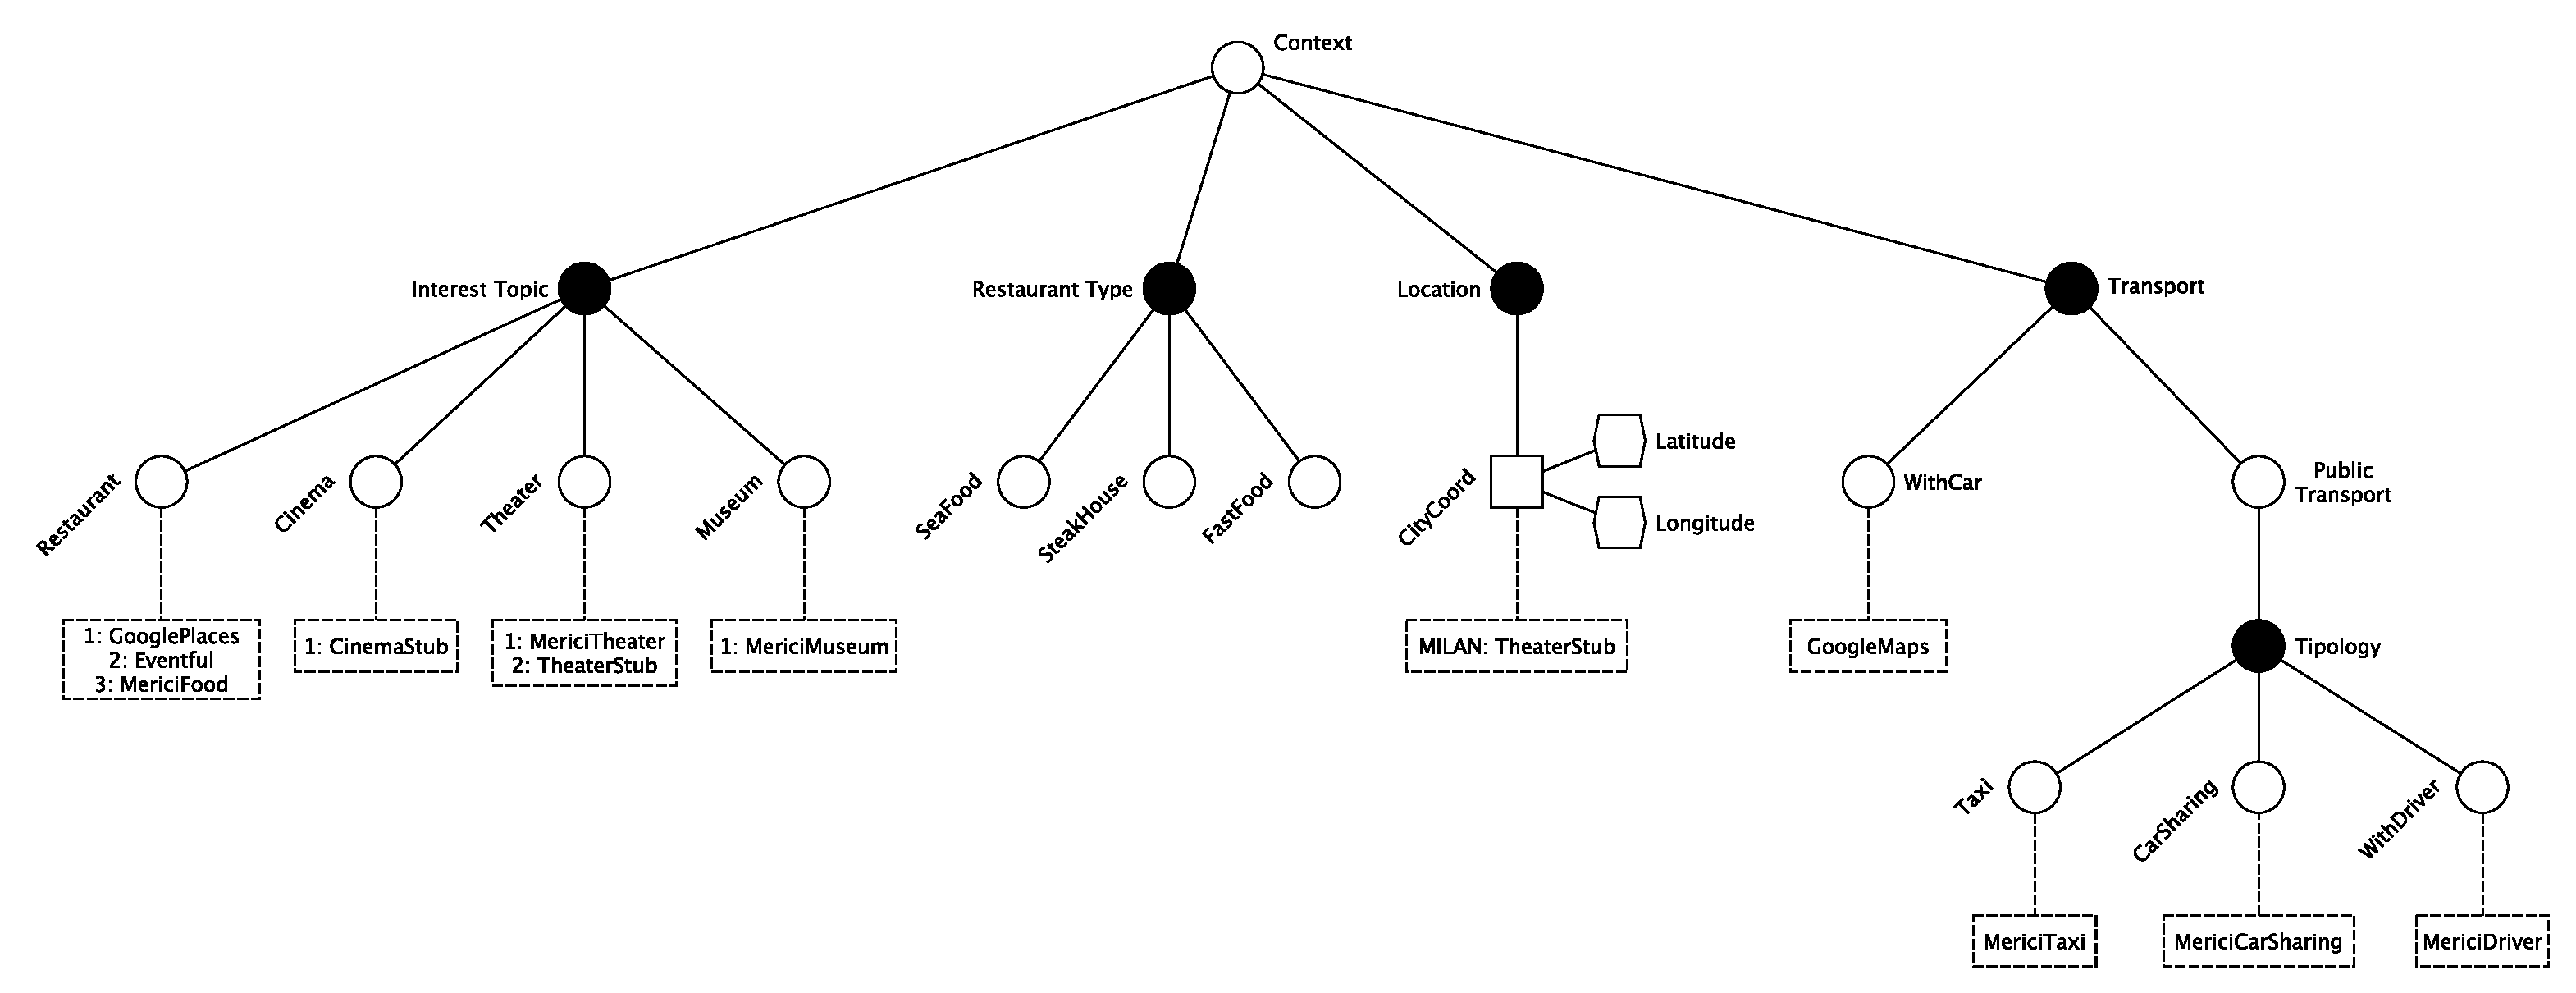
\includegraphics[width=\textwidth]{4-metodologia/Immagini/associazioni-cdt.png}
	\caption{Associazione dei servizi al CDT}\label{fig:associazione-servizi-cdt}
\end{figure}

Come si pu� notare dalla Figura \ref{fig:associazione-servizi-cdt}, le operazioni vengono associate ai nodi di tipo \virgolette{valore} o \virgolette{attributo}. Nel primo caso l'operazione viene aggiunta all'elenco di operazioni che ogni nodo definisce, nel secondo caso � necessario associare a quale/i valore/i associare l'operazione (es.: per il campo \virgolette{Citt�} bisogna definire il nome della citt�, invece per l'attributo \virgolette{Coordinate} � necessario specificare la latitudine e longitudine del luogo). Generalmente le associazioni vengono effettuate nei nodi foglia; resta tuttavia possibile effettuare delle associazioni anche nei nodi che hanno dei figli, quando per esempio un servizio copre diverse categorie e non ha senso che sia scelto in una sola di esse.

Per quanto riguarda i \emph{servizi primari}, quando vengono associati ad un determinato contesto viene definito anche un indice di \emph{priorit�}: questo valore � un numero intero, a partire da 1 e crescente all'interno del singolo nodo. Definisce l'importanza che il servizio assume in quel determinato contesto e verr� utilizzato nella fase di selezione dei servizi illustrata nel Capitolo \ref{sec:primary-service-selection}. Questo indicatore ha senso di essere utilizzato esclusivamente nei \emph{nodi valore}, in quanto contengono una raccolta generica di servizi, mentre per i \emph{nodi attributo} non � necessario, in quanto l'ordinamento all'interno di una categoria di attributi non � sempre univoca. Se si prende per esempio un elenco di servizi associati ad una citt� tramite le sue coordinate geografiche, si pu� considerare come indice di priorit� la lontananza rispetto all'utente, che pu� essere calcolata solamente a runtime e pu� variare spesso.

%bisogna parlare degli interest topic?
Per i \emph{servizi di supporto} non � sempre necessario definire le associazioni con i nodi del CDT. Alcuni servizi di supporto possono essere richiamati in modo statico quando non necessitano del contesto per essere scelti (es.: servizi generici come Wikipedia\footnote{\url{https://en.wikipedia.org/wiki/Main_Page}} o Flickr\footnote{\url{https://www.flickr.com/}}). Per altri servizi, come per esempio quelli relativi ai mezzi di trasporto, � invece necessario basarsi sul contesto per selezionare il servizio pi� idoneo alla situazione. Per esempio, se un utente specifica che non dispone di un'auto e che si trova a Milano, allora il sistema proporr� i mezzi di trasporto pubblici presenti nella citt�, insieme all'elenco di altri tipologie di trasporto come i taxi o il car sharing. In questo caso � dunque necessario, come per i servizi primari, definire le associazioni delle operazioni con i nodi del CDT. Il processo di associazione � simile a quello dei servizi primari, la principale differenza risiede nel fatto che non bisogna specificare la priorit� dei servizi, mentre le altre assunzioni rimangono valide.

\section{CDT su misura per gli utenti}

\textcolor{red}{Divisione tra schema universale e tailored}\\

Il modello del CDT definito nella Sezione \ref{sec:associazione-servizi-cdt} viene chiamato \emph{CDT universale}, in quanto rappresenta lo schema pi� completo del quale il sistema pu� disporre.

\section{Mashup Design\label{sec:mashup-design}}

\textcolor{red}{Spiegare lo schema per la generazione dinamica delle schermate\\
Descrizione web app per la creazione degli schemi}

\section{Dove eseguire le query verso i servizi?}
%Non sono sicuro di mettere questa sezione qui, poi vediamo dove spostarla
Uno dei primi problemi che abbiamo dovuto affrontare � quello di pensare a come eseguire le richieste verso i servizi esterni. Le due principali soluzioni che vengono adottate nelle piattaforme di mashup per dispositivi mobile sono \emph{Server Mashup} e \emph{Cold Client Mashup} \textcolor{red}{(trovare qualche reference qui?)}
Nel Server Mashup tutte le operazioni vengono eseguite sul server, precisamente, dato un mashup, si occupa di tutte le operazioni di richiesta, integrazione e composizione dei dati, portando tutta la complessit� delle operazioni sul server.
Il Cold Client Mashup, invece, lo schema di mashup viene scaricato sul dispositivo, quindi le operazioni di richiesta, integrazione e composizione vengono eseguite direttamente dal dispositivo.
Entrambe le soluzioni non sono molto bilanciate. Ha senso utilizzare il server come unico componente che esegue tutte le operazioni sui dati e usare l'app mobile solo come semplice browser dove a partire da una richiesta ottengo una o un insieme di risposte? Oppure ha senso spostare tutta la complessit� computazionale sul dispositivo mobile?
Data la crescente potenza di calcolo dei processori destinati al comparto mobile la tentazione di far fare molte operazioni anche complesse al dispositivo mobile � molto forte, tuttavia questo non risolve diverse problematiche.
I servizi non � detto che abbiano i medesimi tempi di risposta, quindi l'applicazione per eseguire una query dovrebbe avere una propria cache. Questo inoltre aggiunge un problema con le API keys dei servizi, che nel caso in cui fossero limitate, porterebbero ad eseguire tante richieste, portando a costi maggiori o a un esaurimento di queries verso il servizio. Questo problema verrebbe risolto utilizzando un unico punto di esecuzione delle query con un meccanismo di caching, in modo da evitare ripetizioni di richieste, tentando di ridurre l'incidenza di questo problema.
Esistono altri due problemi, i quali sono legati all'autonomia e all'utilizzo dei dati del mobile device. L'esecuzione di richieste e operazioni sui dati porta ovviamente a un maggiore consumo di risorse hardware di calcolo e di telecomunicazione, consumando maggiormente la batteria integrata. Con una query unica e con i dati gi� aggregati ovviamente riduce il consumo delle risorse energetiche e dei dati in connessione mobile.

\section{Architettura utilizzata\label{sec:architettura-sistema}}

\begin{figure}[h]
	\centering
	\includegraphics[width=\textwidth]{4-metodologia/Immagini/ArchitectureGen2016.png}
	\caption{Architettura del sistema}\label{fig:architettura-sistema}
\end{figure}

Come evidenziato nella figura \ref{fig:architettura-sistema}, l'architettura finale del sistema CAMUS � composta da tre parti, ognuna delle quali � collegata con l'utente finale del sistema.

\begin{enumerate}
	\item \textbf{Server} Il server � l'endpoint al quale si interfaccia l'amministratore del sistema, il quale ha una visione maggiore della complessit� del sistema. Ha il compito di aggiungere i servizi disponibili compilando un campo Qui vengono registrati i servizi poi che vengono mappati dall'esperto nelle \emph{Web App} 
	Data una query proveniente dall'applicazione mobile, comprendente il contesto e i dati che ha bisogno il client,il server seleziona i servizi da contattare tramite il \emph{Service Selector}, esegue le query verso i servizi esterni e compone i risultati a seconda a seconda delle regole associate a ciascun servizio.
	
	\item \textbf{Web App} Le web app sono collegate all'esperto di settore che compone l'applicazione mobile. Questo attore non � necessariamente un esperto di informatica e della tecnologia utilizzata, quindi ha bisogno di un astrazione maggiore rispetto all'amministratore. Sono disponibili due funzionalit� di base: una permette di associare i servizi al CDT dell'utente, mentre l'altra permette di creare i mashup per le pagine dell'applicazione, collegando i termini con i componenti che verranno poi renderizzati nell'applicazione.
	
	\item \textbf{App Mobile} La app mobile � l'interfaccia dell'utente finale con il sistema. Essa ha il compito di renderizzare i mashup definiti dall'esperto e di permettere all'utente di inserire il proprio contesto per richiedere al server i risultati associati ad esso. I dati occorrenti per generare un contesto possono essere anche aggiunti utilizzando i sensori del dispositivo, come il GPS o l'ora corrente.
\end{enumerate}








\chapter{Progettazione di dettaglio e implementazione del backend\label{ch:implementazione-backend}}

Questo capitolo illustra nel dettaglio la realizzazione del \emph{backend} della piattaforma CAMUS. Il capitolo si apre con l'esposizione e la descrizione delle entità principali. Alcune di queste entità meritano però una sezione a parte, data la loro complessità. In particolare vengono analizzate dettagliatamente il descrittore dell'albero del contesto e il descrittore dei servizi. Verrà fornita una descrizione degli attributi che li caratterizzano, con l'ausilio di esempi per chiarire meglio i concetti. Successivamente viene mostrato lo schema logico del \emph{backend} e vengono analizzati i dettagli implementativi dei singoli componenti. Una sezione verrà dedicata all'\emph{endpoint GraphQL}, che permette alle applicazioni esterne di eseguire le attività messe a disposizione dal \emph{backend}. Il capitolo termina con la documentazione relativa la configurazione del sistema, che permette la definizione di alcuni parametri utilizzati nella fase di esecuzione per modificarne il comportamento. Una configurazione può essere definita tramite variabili d'ambiente o file di configurazione. Verranno descritte entrambe le possibilità.

\section{Schema del database\label{sec:schema-database}}

\begin{figure}[p]
	\centering
	\includegraphics[height=\textwidth, angle=90]{5-implementazione-backend/Immagini/schema_er_db.png}
	\caption{Diagramma ER del database}\label{fig:schema-er-db}
\end{figure}

La base di dati viene utilizzata principalmente per garantire la persistenza di tre elementi: \emph{i)} il descrittore dei servizi, \emph{ii)} l'albero del contesto e \emph{iii)} le associazioni tra operazioni e nodi del CDT.

Queste entità permettono al sistema di svolgere le attività principali. In quanto oggetti complessi verranno descritti nel dettaglio nelle sezioni successive, per metterne in risalto le caratteristiche e le peculiarità. In Figura \ref{fig:schema-er-db} viene mostrato il modello \emph{Entità-Relazione} che sta alla base di CAMUS.

Sono presenti entità per la memorizzazione delle informazioni sull'u\-ten\-te. Un'altra entità importante riguarda i \emph{mashup}, che vengono associati all'utente per permettere la definizione di schemi personalizzati. I dettagli sulla composizione di questi schemi verranno esposti nella Sezione \ref{sec:struttura-schemi-mashup}.

Una volta definito il modello ER è necessario passare alla realizzazione dello \emph{schema logico} del database, quello che verrà effettivamente utilizzato nell'im\-ple\-men\-ta\-zio\-ne. Non esistendo uno standard per realizzare uno schema di questo tipo per i database non relazionali è stato scelto di utilizzare un \emph{diagramma delle classi} per rappresentare i \emph{documenti} che compongono il database. Ogni classe viene intesa come un documento e i collegamenti evidenziati con una linea continua rappresentano i sottodocumenti. Le linee tratteggiate indicano le referenze tra i vari documenti.

In Figura \ref{fig:schema-logico-db} viene mostrato lo schema logico utilizzato per CAMUS.

\begin{figure}[!b]
	\centering
	\includegraphics[width=\textwidth]{5-implementazione-backend/Immagini/schema_logico_db.png}
	\caption{Schema logico del database}\label{fig:schema-logico-db}
\end{figure}

\section{Descrittore dell'albero di contesto\label{sec:descrittore-albero-contesto}}

Nella Sezione \ref{sec:context-dimension-model} è stato esposto il modello teorico del \emph{Context Dimension Tree} mentre in questa sezione si vuole mettere in risalto come l'albero di contesto viene descritto nel sistema. Sono state effettuate diverse semplificazioni per agevolare la memorizzazione e il recupero delle informazioni dai vari nodi che compongono l'albero. Nelle seguenti sottosezioni vengono analizzati nel dettaglio i singoli oggetti che formano un albero di contesto.

\subsection{Radice\label{sec:radice-cdt}}

Questo oggetto rappresenta la radice di un albero di contesto. \upe composto dai seguenti parametri:

\begin{itemize}
	\item \textbf{User Id}
	L'elenco degli identificativi degli utenti ai quali questo albero è associato. Viene lasciata la possibilità di definire più utenti perché uno stesso albero può essere valido per più utenti con un profilo simile
	\item \textbf{Context}
	Contiene i \emph{nodi} che compongono l'albero. Per una descrizione approfondita si fa riferimento alla Sezione \ref{sec:nodo-cdt}
	\item \textbf{Default Values}
	Vengono elencati tutti i valori che l'\emph{esperto di settore} ha specificato siano sempre validi per gli utenti ai quali questo albero viene associato. \upe composto dal nome della \emph{dimensione} e dal relativo \emph{valore} che assume
\end{itemize}

Viene inoltre definito un \emph{CDT Globale}, utilizzato come base per la creazione di quelli specifici per ogni utente. Questo albero ha la particolarità che non è associato a nessun utente.

\subsection{Nodi\label{sec:nodo-cdt}}

Questo oggetto rappresenta un nodo dell'albero. In particolare vengono rappresentati solamente i nodi di tipo \emph{dimensione} tramite oggetti dedicati, mentre i nodi \emph{contesto} e \emph{parametro} vengono rappresentati come sottocomponenti. Ogni nodo possiede i seguenti attributi:

\begin{itemize}
	\item \textbf{Name}
	Il nome del nodo dimensione
	\item \textbf{For}
	Descrive la tipologia di nodo, utilizzata per assegnare un peso utile nella fase di \emph{selezione delle operazioni} e per attribuire un valore ai parametri nella fase di \emph{invocazione dei servizi}. I valori ammessi sono \emph{filter}, \emph{parameter} o \emph{ranking}. Vengono inoltre ammesse le combinazioni \emph{filter}|\emph{parameter} e \emph{ranking}|\emph{parameter}: un nodo può essere solamente di tipo \emph{filter} o \emph{ranking}, al fine dell'assegnamento dei pesi, mentre può essere anche di tipo \emph{parameter}, in quanto indica che verrà utilizzato anche nella fase di composizione delle query. Se viene definito il tipo \emph{parameter} devono essere assegnati diversi \emph{parametri}, per specificarne le caratteristiche
	\item \textbf{Values}
	Elenca i possibili valori che può assumere il nodo. Questo elenco corrisponde ai nodi di tipo \emph{contesto} del modello del CDT
	\item \textbf{Parameters}
	L'elenco dei parametri associati al nodo. Per ulteriori dettagli su questo oggetto si fa riferimento alla Sezione \ref{sec:parametro-cdt}
	\item \textbf{Parents}
	Contiene l'elenco di tutti i nodi dimensione dai quali discende il nodo corrente. Viene utilizzato per effettuare l'unione delle sottodimensioni di un nodo
\end{itemize}

Nel Listato \ref{lst:esempio-nodo-cdt} viene mostrato un esempio di nodo.

\begin{listing}[H]
	\inputminted{json}{5-implementazione-backend/Codice/esempio_nodo_cdt.json}
	\caption{Esempio di nodo del CDT}
	\label{lst:esempio-nodo-cdt}
\end{listing}

\subsection{Parametri dei nodi\label{sec:parametro-cdt}}

Questo oggetto definisce i parametri che sono associati a un nodo dimensione. Corrisponde ai nodi di tipo \emph{parametro} del modello del CDT. I parametri vengono utilizzati per permettere all'utente di specificare dei valori di sua scelta (es.: località). \upe composto dai seguenti campi:

\begin{itemize}
	\item \textbf{Name}
	Il nome del parametro
	\item \textbf{Type}
	Il/I formato/i del dato che vengono accettati
	\item \textbf{Fields}
	Questo elenco permette di definire dei campi che vanno ulteriormente a specificare il parametro. Un esempio viene dato dal parametro \virgolette{Luogo}, che può essere specializzato nei campi \virgolette{Latitudine} e \virgolette{Longitudine}
\end{itemize}

Nel Listato \ref{lst:esempio-parametro-cdt} viene mostrato un esempio di parametro.

\begin{listing}[H]
	\inputminted{json}{5-implementazione-backend/Codice/esempio_parametro_cdt.json}
	\caption{Esempio di parametro associato a un nodo}
	\label{lst:esempio-parametro-cdt}
\end{listing}

\section{Descrittore dei servizi\label{sec:descrittore-servizi}}

Affinché il sistema possa effettuare le richieste è necessario che sia presente una formato per descrivere le caratteristiche di ogni servizio (es.: l'indirizzo verso il quale effettuare la richiesta, i parametri da inserire, ecc.). Per questo motivo è stato introdotto l'utilizzo di un \emph{descrittore dei servizi} in grado di specificare tutte le possibili configurazioni che i servizi possono richiedere. I \emph{descrittori} non sono altro che configurazioni dei servizi espressi tramite file JSON. Di seguito verranno analizzati nel dettaglio tutti i campi che compongono il descrittore. \upe stata separata la definizione delle informazioni generali del servizio dalle informazioni di dettaglio delle operazioni che espone. Il risultato sono due oggetti, uno di \virgolette{descrizione generale del servizio} e un \virgolette{descrittore delle operazioni}. Nelle seguenti sezioni verranno analizzati gli attributi di entrambi gli oggetti.

\subsection{Descrizione generale del servizio\label{sec:oggetto-principale-servizi}}

\upe il punto di partenza per la descrizione di un servizio. Comprende i seguenti campi:

\begin{itemize}
	\item \textbf{Name}
	Il nome del servizio
	\item \textbf{Description}
	Fornisce una descrizione delle funzionalità del servizio
	\item \textbf{Protocol}
	Definisce la tipologia con la quale accedere al servizio. Può assumere i valori \virgolette{rest}, \virgolette{query} o \virgolette{custom}, per specificare rispettivamente che il servizio viene invocato secondo il protocollo REST, viene composta una query con parametri o è necessario invocare un metodo particolare per l'accesso
	\item \textbf{Base Path}
	Rappresenta l'indirizzo di base del servizio. A partire da questo indirizzo verrà composto quello completo aggiungendo in coda i percorsi specifici delle \emph{operazioni} richieste. Non deve essere inserita al termine nessuno slash (\virgolette{/})
\end{itemize}

Nel Listato \ref{lst:esempio-descrittore-servizio} viene mostrato un esempio di oggetto principale del servizio.

\begin{listing}[H]
	\inputminted{json}{5-implementazione-backend/Codice/esempio_descrittore_servizio.json}
	\caption{Esempio di servizio}
	\label{lst:esempio-descrittore-servizio}
\end{listing}

\subsection{Descrittore delle operazioni\label{sec:descrittore-operazioni}}

Rappresenta le operazioni che sono messe a disposizione dal servizio. Un'o\-pe\-ra\-zio\-ne viene descritta dai seguenti campi:

\begin{itemize}
	\item \textbf{Service}
	Contiene il riferimento al \emph{descrittore generale del servizio} associato all'operazione. Un'operazione può essere collegata esclusivamente ad un solo servizio
	\item \textbf{Name}
	Il nome dell'operazione
	\item \textbf{Type}
	Rappresenta la tipologia dell'operazione. Un'operazione può essere \emph{primaria} o di \emph{supporto}. Questa distinzione viene utilizzata principalmente per permettere la catalogazione delle operazioni da mostrare nelle web app
	\item \textbf{Description}
	La descrizione dell'attività svolta dall'operazione
	\item \textbf{Path}
	Il percorso specifico per richiamare l'operazione. Questo valore viene aggiunto al \emph{Base Path} del servizio. Deve essere sempre preceduto da una slash (\virgolette{/})
	\item \textbf{Protocol}
	Permette di ridefinire il protocollo utilizzato esclusivamente per l'operazione corrente. \upe utile nei casi in cui un'operazione, per una qualsiasi ragione, utilizzi un paradigma di composizione della query diverso da quello specificato dal servizio. Per esempio, viene utilizzato per mappare gli \virgolette{intent} su diversi sistemi operativi dei dispositivi, che hanno diverse regole di composizione. Oltre alle tipologie definite per i \emph{servizi} supporta anche il protocollo \virgolette{android}
	\item \textbf{Store Link}
	Utilizzato esclusivamente per i servizi di supporto, permette di definire il link nello store di riferimento per scaricare l'app necessaria a utilizzare l'intent associato
	\item \textbf{Bridge Name}
	Questo campo è opzionale, definisce il nome del bridge con la logica necessaria per invocare il servizio. \upe obbligatorio il suo utilizzo quando per il servizio viene utilizzato il protocollo \emph{custom}
	\item \textbf{Parameters}
	Definisce l'elenco dei parametri accettati in ingresso dall'o\-pe\-ra\-zio\-ne. Per ulteriori dettagli su questo oggetto si fa riferimento alla Sezione \ref{sec:descrittore-parametri}
	\item \textbf{Headers}
	Permette di specificare gli attributi da aggiungere all'header della richiesta. Vengono utilizzati i campi \virgolette{name} per specificare il nome dell'at\-tri\-bu\-to e \virgolette{value} per specificarne il valore
	\item \textbf{Response Mapping}
	Serve per definire le regole di associazione per mappare la risposta del servizio coi termini semantici utilizzati dal sistema. Maggiori dettagli su questo oggetto vengono discussi nella Sezione \ref{sec:descrittore-risposta}
	\item \textbf{Pagination}
	Serve a raccogliere gli attributi necessari per gestire la paginazione specifica di ogni servizio. Sono supportati meccanismi di paginazioni basati sul \emph{numero di pagina} o su \emph{token}. Questo oggetto viene analizzato nel dettaglio nella Sezione \ref{sec:descrittore-paginazione}
\end{itemize}

Nel Listato \ref{lst:esempio-descrittore-operazione} viene mostrato un esempio di operazione. Nel campo \virgolette{service} viene inserito il nome del servizio associato al posto del suo identificativo per maggiore chiarezza.

\begin{listing}[H]
	\inputminted{json}{5-implementazione-backend/Codice/esempio_descrittore_operazione.json}
	\caption{Esempio di operazione}
	\label{lst:esempio-descrittore-operazione}
\end{listing}

\subsection{Parametri delle operazioni\label{sec:descrittore-parametri}}

Quest'oggetto definisce i parametri in ingresso di un'operazione. I parametri generalmente sono composti da due campi: uno ne definisce il \emph{nome} e l'altro il rispettivo \emph{valore}. In alcuni casi vengono accettati più valori, quindi il descrittore deve dunque essere in grado di gestire questa situazione. Un ulteriore compito affidato a questo oggetto è quello di acquisire il valore di un determinato parametro dal \emph{contesto}. Viene inoltre fornito un semplice sistema di traduzione dei dati acquisiti dal contesto, per permettere le trasformazioni verso un valore idoneo per l'operazione corrente. Infine, soprattutto per le operazioni di \emph{supporto}, viene permessa un'associazione del parametro verso uno o più \emph{termini semantici}, per permettere all'app mobile di conoscere l'attributo dove andare a recuperare il valore concreto a run-time. Nello specifico, l'oggetto è così composto:

\begin{itemize}
	\item \textbf{Name}
	Il nome del parametro. Questo campo è \emph{obbligatorio}, in quanto definisce il nome che verrà utilizzato per comporre la query per richiedere i dati
	\item \textbf{Description}
	La descrizione della tipologia del parametro
	\item \textbf{Required}
	Specifica se il parametro corrente è obbligatorio o meno in una richiesta. Non definire questo attributo equivale ad assegnargli valore \emph{false}
	\item \textbf{Type}
	Definisce il \emph{tipo} di dato che l'operazione si aspetta di ricevere. Le principali tipologie di dato che vengono inviate verso i servizi sono \emph{stringhe}, \emph{numeri} o \emph{date}
	\item \textbf{Default}
	Indica un valore predefinito per il parametro. Questo campo è particolarmente utile per la web app relativa al \emph{Visual Mapping}, in quanto permette di ricevere degli esempi di risposta dei servizi da mostrare all'utente
	\item \textbf{Collection Format}
	Questo campo definisce il \emph{separatore} da utilizzare nel caso siano presenti più valori per il parametro. Sono accettati i seguenti quattro separatori: \emph{i)} csv, comma separated values; \emph{ii)} ssv, space separated values; \emph{iii)} tsv, tab separated values; \emph{iv)} pipes. Se non specificato viene utilizzato di default il tipo \emph{csv}
	\item \textbf{Mapping CDT}
	Definisce uno o più nodi dell'albero di contesto dove andare ad acquisire il valore ricevuto dalla mobile app. Nel caso vengano associati più di un nodo viene seguito l'ordine di definizione nella fase di composizione della query
	\item \textbf{Mapping Term}
	Definisce uno o più termini semantici da associare al parametro. Questi termini vengono utilizzati a run-time per andare ad acquisire il valore del parametro dalle risposte ricevute dai servizi primari
	\item \textbf{Translate}
	Permette delle semplici trasformazioni dei valori acquisiti dall'al\-be\-ro di contesto per renderli conformi a quelli accettati dal servizio. \upe formato dai campi \virgolette{from} e \virgolette{to}, che specificano rispettivamente il valore di \emph{origine} e quello \emph{tradotto}. Vengono definite tante traduzioni quanti sono i valori che può assumere il rispettivo nodo del CDT
\end{itemize}

Nel Listato \ref{lst:esempio-descrittore-parametro} viene mostrato un esempio di parametro.

\begin{listing}[H]
	\inputminted{json}{5-implementazione-backend/Codice/esempio_descrittore_parametro.json}
	\caption{Esempio di parametro}
	\label{lst:esempio-descrittore-parametro}
\end{listing}

\subsection{Formato della risposta\label{sec:descrittore-risposta}}

In quest'oggetto sono definite le regole con le quali vengono trasformate le risposte ricevute dal servizio nel formato interno CAMUS, dove ogni attributo viene associato a un rispetto \emph{termine semantico} che ne definisce il contenuto. In particolare, vengono utilizzati i seguenti campi:

\begin{itemize}
	\item \textbf{List}
	Definisce l'attributo che contiene l'elenco dei risultati. \upe utile nei casi in cui la risposta, oltre ai risultati, contiene al suo interno anche dei metadati relativi l'interrogazione. Se non specificato si assume che l'elenco dei risultati si trovi nella radice della risposta
	\item \textbf{Items}
	Permette di mappare i vari campi che compongono ogni oggetto dei risultati. In particolare vengono definiti il \virgolette{percorso} dal quale recuperare il valore e il \virgolette{termine semantico} da associare. I campi senza un'associazione saranno ignorati dal processo di trasformazione e le relative informazioni andranno perdute. \upe necessario dunque effettuare l'operazione di mapping delle risposte con attenzione, in modo da non trascurare informazioni importanti
	\item \textbf{Functions}
	Viene permesso l'utilizzo di funzioni specifiche per trasformare i valori. Questa funzione riceve in ingresso il parametro \virgolette{value}, che rappresenta il valore corrente del campo, e deve restituire il nuovo valore che verrà sostituito a quello originale. Oltre alla funzione specifica è necessario definire anche l'\emph{attributo} sul quale eseguire questa trasformazione. L'attributo equivale al \emph{termine semantico} definito nel punto precedente
\end{itemize}

Nel Listato \ref{lst:esempio-formato-risposta} viene mostrato un esempio di formato di risposta.

\begin{listing}[H]
	\inputminted{json}{5-implementazione-backend/Codice/esempio_formato_risposta.json}
	\caption{Esempio di formato di risposta}
	\label{lst:esempio-formato-risposta}
\end{listing}

\subsection{Paginazione\label{sec:descrittore-paginazione}}

In quest'oggetto vengono descritti gli attributi necessari per gestire la paginazione delle risposte. In particolare il sistema è in grado di gestire due tecniche di paginazione, quella basata sul \emph{numero di pagina} e quella che utilizza dei \emph{token} per richiamare le pagine. L'oggetto è composto dai seguenti campi:

\begin{itemize}
	\item \textbf{Attribute Name}
	Specifica il nome del parametro da aggiungere alla query per richiamare una specifica pagina
	\item \textbf{Type}
	Definisce il meccanismo di paginazione da utilizzare. Sono ammessi due valori: \virgolette{number}, per la paginazione basata sul numero di pagine, e \virgolette{token}, per quella che sfrutta i token per richiamare le pagine successive
	\item \textbf{Token Attribute}
	Serve per definire dove andare a leggere nella risposta il token relativo alla pagina successiva
	\item \textbf{Page Count Attribute}
	Definisce l'attributo che fornisce l'informazione del numero di pagine totale che possono essere richieste
\end{itemize}

Nel Listato \ref{lst:esempio-descrittore-paginazione} viene mostrato un esempio di descrittore della paginazione.

\begin{listing}[H]
	\inputminted{json}{5-implementazione-backend/Codice/esempio_descrittore_paginazione.json}
	\caption{Esempio di descrittore della paginazione}
	\label{lst:esempio-descrittore-paginazione}
\end{listing}

\section{Componenti\label{sec:componenti-backend}}

\begin{figure}[p]
	\centering
	\includegraphics[height=\textwidth, width=\textheight, angle=90]{5-implementazione-backend/Immagini/diagramma_classi_backend.png}
	\caption{Diagramma delle classi del backend}\label{fig:class-diagram-backend}
\end{figure}

Come già evidenziato nella Sezione \ref{sec:architettura-backend}, l'architettura del backend è composta da diversi \emph{componenti}. Questa soluzione è stata adottata per via dell'elevata flessibilità che garantisce. Ogni componente è specializzato in un compito preciso e il concatenamento di più componenti permette di realizzare funzionalità più complesse per produrre il risultato desiderato. Per svolgere le principali attività vengono dunque create delle \emph{pipeline}, dove il risultato di un componente viene acquisito e ulteriormente elaborato dal successivo.

Altra caratteristica importante è l'assenza di informazioni sullo stato in ogni componente. Una richiesta nasce nel momento in cui l'utente conferma l'attività e muore una volta che viene evasa. La ragione principale di questa scelta risiede nel fatto che sarebbe oneroso lato backend gestire tutte le informazioni della moltitudine di utenti che sono connessi al sistema. Inoltre mantenere uno stato limiterebbe la scalabilità del sistema, in quanto se un utente inizia la sessione su di un determinato server dovrà continuare sempre su quello, rendendo complicato il bilanciamento dei carichi tra le diverse macchine.

A questo punto è necessaria una importante precisazione: per la gestione della paginazione è necessario l'utilizzo di alcune informazioni sullo stato. Questa affermazione può sembrare un controsenso rispetto a ciò che è stato esposto nel paragrafo precedente. \upe dunque essenziale definire in modo dettagliato cosa si intende per \emph{stato}. La principale differenza consiste nel \emph{dove} vengono salvate le informazioni. Nel paragrafo precedente, ogni volta che si menzionava il concetto di \emph{stato}, si intendevano tutte le informazioni relative l'utente salvate all'\emph{interno} dei componenti, sotto forma di variabile. Questa soluzione può essere un collo di bottiglia non indifferente, in quanto tutte le richieste che nascono in una determinata macchina dovranno essere gestite esclusivamente da essa. Si è adottata quindi una soluzione differente: i \emph{componenti} non mantengono al loro interno alcuna informazione riguardo lo stato, che verrà invece memorizzato e reso disponibile da un servizio esterno. Questa soluzione permette a tutti i componenti che ne hanno esigenza di andare a recuperare le informazioni sullo stato da una sorgente comune, che non limita la scalabilità del sistema. Questo servizio può a sua volta offrire dei sistemi di \emph{clustering} per aumentare le perfomance in situazioni di elevato carico.

In CAMUS questa attività viene svolta da \emph{Redis}, che è stato selezionato per l'elevata rapidità nell'evadere le richieste e nella possibilità di associare un periodo di vita alle informazioni che vengono memorizzate. Viene ipotizzato che dopo un intervallo di tempo nel quale l'utente non effettua più interazione sulla sessione, essa può ritenersi estinta e i suoi dati eliminati.

Per gestire le funzionalità del server viene utilizzato il \emph{web framework} \emph{ExpressJS}\footnote{ExpressJS: \url{http://expressjs.com/}}. \emph{ExpressJS} è un \emph{framework} molto leggero, che mette a disposizione le funzionalità base affinché un server sia operativo. Ha la potenzialità di avere un ottimo sistema di \emph{middleware}, che permette di utilizzare altre funzionalità più avanzate.

Per \emph{GraphQL} viene utilizzata l'implementazione specifica per \emph{Javascript} rilasciata da \emph{Facebook}\footnote{GraphQL-js: \url{https://github.com/graphql/graphql-js}} e l'estensione di \emph{Relay}\footnote{Relay-GraphQL: \url{https://github.com/graphql/graphql-relay-js}} per gestire le connessioni. Affinché gli schemi di \emph{GraphQL} possano essere esposti dal server si sfrutta l'apposito \emph{middleware} \emph{Express-GraphQL}\footnote{Express-GraphQL: \url{https://github.com/graphql/express-graphql}}.

\emph{MongoDB} non possiede una struttura dello schema del database definita a priori. Per garantire coerenza coi dati memorizzati si è scelto di utilizzare un \emph{Object Relational Mapping} (ORM)\footnote{Object Relational Mapping: \url{https://it.wikipedia.org/wiki/Object-relational_mapping}}. Un ORM fornisce un livello di astrazione superiore a un driver nativo e permette di specificare come gli oggetti vengono mappati nel database e viceversa, definendo implicitamente uno schema del database. In particolare, per il progetto CAMUS è stato utilizzato un ORM specifico per Node.js di nome \emph{mongoose}\footnote{MongooseJS: \url{http://mongoosejs.com/}}.

Infine, per interfacciare Node.js con l'istanza di Redis in esecuzione viene utilizzato il modulo \emph{ioredis}\footnote{ioredis: \url{https://github.com/luin/ioredis}}.

In Figura \ref{fig:class-diagram-backend} viene mostrato il diagramma delle classi di tutti i componenti che formano il backend del sistema. Nelle seguenti sottosezioni verranno analizzate nel dettaglio le attività svolte e i dettagli implementativi dei componenti principali del sistema.

\subsection{Provider\label{sec:provider}}

Il \emph{Provider} rappresenta il punto di accesso ai database. \upe realizzato seguendo il pattern \emph{singleton}, che prevede una singola istanza della classe in comune per tutti i componenti. Le varie classi che necessitano di accedere al database possono recuperare l'istanza corrente tramite il metodo statico \emph{getInstance()}. Durante l'inizializzazione si occupa di creare le connessioni verso MongoDB e Redis. Implementa tutti i metodi necessari per recuperare le informazioni dal database e centralizza tutte le query in un singolo punto, in modo che gli altri componenti del sistema non debbano preoccuparsi di comporre le clausole. Inoltre, visto che diversi metodi vengono utilizzati da più componenti, si evitano duplicazioni di codice che provocano una riduzione della manutenibilità del sistema, in quanto una modifica a un metodo dovrebbe essere ripetuta più volte.

I metodi sono stati raggruppati in sei categorie, in base alla funzionalità:

\begin{enumerate}
	\item \textbf{CDT Methods}
	Mette a disposizione le funzioni necessarie a recuperare gli alberi di contesto. Possono essere cercati tramite identificativo, se si vuole acquisire un albero specifico, oppure tramite utente, se si vuole recuperare il suo CDT personalizzato
	\item \textbf{Service Descriptor Methods}
	Definisce le funzioni che vengono utilizzate per acquisire i descrittori dei servizi. I due oggetti, \virgolette{descrizione generale del servizio} e \virgolette{descrittore delle operazioni} vengono automaticamente integrati a formare un unico oggetto
	\item \textbf{Primary Service Methods}
	Fornisce le funzioni di ricerca delle associazioni tra i nodi del CDT e le operazioni primarie. Il metodo principale riguarda la ricerca delle coppie {<}dimensione, valore{>} definite dalle \emph{dimensioni} del contesto e i relativi \emph{valori}. Possono entrare a far parte di questa categoria anche i metodi di ricerca specializzati, cioè tutte le funzioni che necessitano di logiche particolari per recuperare le associazioni. Un esempio è fornito dalla \emph{ricerca tramite coordinate}: è presente un metodo che sfrutta le capacità di \emph{MongoDB} di eseguire \emph{query geospaziali}
	\item \textbf{Support Service Methods}
	Implementa i metodi di ricerca delle associazioni tra i nodi del CDT e le operazioni di supporto. Rispetta le stesse convenzioni descritte nel punto precedente
	\item \textbf{User Methods}
	Definisce i metodi che vengono utilizzati per l'autenticazione degli utenti e il recupero delle informazioni personali, quali il proprio \emph{albero di contesto} o i \emph{mashup}
	\item \textbf{Redis Methods}
	Vengono messi a disposizione i metodi per richiedere o salvare un oggetto in Redis in base alla chiave che si desidera utilizzare
\end{enumerate}

\subsection{Context Manager\label{sec:context-manager}}

Il \emph{Context Manager} è il componente dedicato alla gestione del contesto. Riceve in ingresso il contesto dell'utente, composto dalle coppie $ {<}dimensione, valore{>} $, e i parametri relativi al proprio albero di contesto. La prima attività svolta è quella di \emph{unire} il contesto dell'utente e la descrizione del CDT presente nel database. Per unione si intende associare a ogni dimensione e parametro il relativo valore ricevuto.

In seguito inizia la fase di creazione del \emph{CDT decorato}. Questa rappresentazione sarà quella che verrà utilizzata da tutti i componenti che seguono il \emph{Context Manager} nella pipeline. Il \emph{CDT decorato} non è altro che il descrittore del CDT in una forma più comoda per essere utilizzata nelle elaborazioni, in quanto cataloga i nodi dell'albero in quattro categorie ben specifiche, che potranno essere semplicemente recuperate dai componenti che ne hanno bisogno senza la necessità di andare ogni volta a leggere l'intero contesto. In particolare, il CDT decorato è composto dalle seguenti categorie:

\begin{itemize}
	\item \textbf{Filter Nodes}
	Sono i nodi di tipo filtro che vengono utilizzati per selezionare le operazioni
	\item \textbf{Ranking Nodes}
	L'elenco dei nodi di tipo ranking che vengono utilizzati per selezionare le operazioni
	\item \textbf{Specific Nodes}
	Sono i nodi che non utilizzano la ricerca standard delle associazioni ma richiedono una ricerca specifica. La definizione di queste due tipologie verrà approfondita nella Sezione \ref{sec:primary-service-selection}
	\item \textbf{Parameter Nodes}
	L'elenco dei nodi dai quali recuperare i valori da utilizzare per la composizione delle query
\end{itemize}

\upe da tenere in considerazione, come precedentemente fatto notare nella Sezione \ref{sec:descrittore-albero-contesto}, che alcuni nodi possono appartenere a più categorie nello stesso tempo. Questa eventualità capita spesso per i nodi che vengono utilizzati sia per filtrare i servizi sia come parametro nella fase di composizione delle query.

Un'altra attività svolta durante la composizione del \emph{CDT decorato} è la ricerca dei nodi figlio. Come definito nella Sezione \ref{sec:associazione-servizi-cdt} le associazioni possono essere specificate sia nei nodi foglia sia in quelli intermedi. \upe importante quindi verificare se un nodo attivo possieda dei figli perché in tal caso anch'essi possono dare un contributo nelle successive fasi di selezione. L'algoritmo per la selezione dei nodi figlio segue la logica esposta nella Sezione \ref{sec:selezione-operazioni}.

\subsection{Primary Service Selection\label{sec:primary-service-selection}}

Il \emph{Primary Service Selection} è il componente dedicato alla ricerca delle operazioni primarie da interrogare. Riceve in ingresso il \emph{CDT Decorato} e produce l'elenco degli \emph{identificativi delle operazioni} selezionate, assieme al relativo \emph{punteggio}.

La prima attività svolta riguarda l'acquisizione delle operazioni che sono associate al contesto corrente. Questa fase viene divisa in due fasi:

\begin{enumerate}
	\item \textbf{Ricerca Standard}
	Viene effettuata ricercando nel database tutte le operazioni che sono associate alle coppie $ {<}dimensione, valore{>} $ attive, ossia i nodi dell'albero selezionati dall'utente. Vengono utilizzati sia i nodi di tipo \emph{filtro} sia quelli di tipo \emph{ranking}, distinguendoli nella fase di assegnamento dei pesi
	\item \textbf{Ricerca Specifica}
	Utilizza dei metodi specifici per ricercare le associazioni. Un esempio è la ricerca delle operazioni tramite \emph{coordinate}, che sfrutta le funzionalità di \emph{MongoDB} di effettuare \emph{query geospaziali}. Le associazioni identificate in questa fase vengono classificate come \emph{ranking}
\end{enumerate}

Una volta recuperate tutte le associazioni, vengono calcolati i punteggi da assegnare ad ognuno, con la procedura descritta nel dettaglio nella Sezione \ref{sec:selezione-operazioni}.

\subsection{Query Handler\label{sec:query-handler}}

Il \emph{Query Handler} è il componente che orchestra le chiamate verso i servizi primari, recupera le risposte e le trasforma nel formato interno. Riceve gli identificativi delle operazioni primarie e ne acquisisce i descrittori completi dal database.

Una volta disponibili può iniziare la fase di richiesta dei dati. Per svolgere questo compito vengono utilizzati diversi \emph{bridge}. \upe possibile così separare l'implementazione specifica del servizio in un altro componente, in modo che i servizi che condividono la medesima logica possano utilizzare lo stesso \emph{bridge}. Il \emph{Query Handler} seleziona dunque il \emph{bridge} idoneo per interrogare il servizio e ne esegue il metodo \emph{executeQuery()}, che si occupa di interrogare il servizio e restituire la risposta ricevuta. Oltre all'elenco dei risultati, viene restituito un oggetto contenente le informazioni sullo stato della paginazione (es.: se sono disponibili ulteriori pagine o il valore per richiamare la pagina successiva), se il servizio possiede una descrizione di come gestire la paginazione.

Quando riceve una risposta provvede a \emph{trasformarla} nel formato interno, basandosi sull'utilizzo di termini semantici che descrivono la semantica degli attributi. Il descrittore contiene al suo interno le informazioni necessarie per effettuare questa trasformazione. In particolare è necessario definire le associazioni per ogni \emph{attributo} rilevante della risposta e il relativo \emph{termine semantico} che lo descrive. Non è obbligatorio definire associazioni per tutti gli attributi di una risposta: se alcuni campi non sono utili possono essere omessi. Una volta terminata la trasformazione viene lasciata la flessibilità di eseguire delle funzioni personalizzate sui valori dei termini in modo da uniformare eventuali dati formattati in modo non idoneo.

Una menzione va fatta alla gestione degli errori. Può capitare che alcuni servizi non siano raggiungibili a causa di problemi di rete. In tal caso il \emph{bridge} restituisce un messaggio di errore al posto della risposta. Il \emph{Query Handler} non tratta gli errori come eventi bloccanti, ma si limita a scrivere questi eventi in un \emph{log}. Infatti, se per esempio devono essere interrogati tre servizi e solo uno dei tre non risponde, non è conveniente interrompere l'intero processo, bensì verranno restituite le risposte ricevute dagli altri due servizi.

Una volta ricevute le risposte dai servizi e terminata la fase di trasformazione, viene creata un'unica lista comprendente tutti gli elementi ricevuti. Vengono in pratica uniti i vettori ricevuti dai diversi servizi. Questo elenco rappresenta il risultato finale, che verrà dato in carico al componente successivo nella catena.

\subsection{Bridge\label{sec:bridge}}

Un \emph{Bridge} è il componente che si occupa di gestire le chiamate verso i servizi esterni e ricevere le risposte. \upe costituito da una classe astratta che deve essere estesa dalle implementazioni specifiche. In questo modo viene lasciata flessibilità di estensione ogni qual volta sia necessaria una logica diversa per invocare un servizio. In particolare viene forzata l'implementazione del metodo \emph{executeQuery()}, che riceve in ingresso il \emph{CDT Decorato} con tutte le informazioni necessarie per per completare i parametri richiesti dal servizio.

Nella sezione seguente viene analizzata l'unica implementazione specifica che viene fornita in dotazione col sistema, quella per l'utilizzo dei servizi di tipo REST.

\subsubsection*{REST Bridge}

Il \emph{REST Bridge} fornisce la logica per interrogare i servizi di tipo REST. La prima attività che svolge è la composizione dell'indirizzo verso il quale il servizio deve essere interrogato. A tal fine viene utilizzato il componente \emph{Query Composer} (Sezione \ref{sec:query-composer}), che è specializzato nell'eseguire questa operazione. In questa fase entra in gioco anche l'informazione sulla prima pagina da interrogare, nel caso in cui quella corrente non sia la prima chiamata che viene effettuata verso il servizio.

Una volta composto l'indirizzo completo, viene effettuata la chiamata verso il servizio. Le risposte ricevute vengono salvate in \emph{cache}, quindi questa attività ha due varianti: se il dato è presente in \emph{cache}, questo viene recuperato e fornito immediatamente in uscita, altrimenti viene interrogato il servizio e il risultato fornito viene salvato in \emph{cache} per utilizzi futuri. I dati restano in \emph{cache} per un determinato periodo di tempo definito a priori dalla configurazione del sistema.

Se il servizio prevede l'utilizzo della paginazione viene analizzata la risposta alla ricerca di informazioni sulla presenza di ulteriori pagine da richiedere. In particolare vengono cercati gli attributi relativi al numero totale di pagine o al \emph{token} per richiamare la pagina successiva, in base alla tipologia implementata dal servizio.

Infine vengono restituite in uscita la risposta del servizio insieme alle eventuali informazioni riguardo la paginazione, che in particolare sono due: \emph{i)} \emph{hasNextPage}, che indica se è presente un'altra pagina; \emph{ii)} \emph{nextPage}, che specifica il numero di pagina o \emph{token} da utilizzare per richiamare la nuova pagina.

Come descritto nella Sezione \ref{sec:query-handler}, nel caso si verifichi un problema durante l'interrogazione del servizio, il \emph{bridge} deve restituire un messaggio d'errore con la motivazione per la quale non è riuscito a completare l'operazione (es.: servizio non raggiungibile, richiesta mal formata, ecc.).

\subsection{Response Aggregator\label{sec:response-aggregator}}

Il \emph{Response Aggregator} entra in gioco una volta che sono stati interrogati tutti i servizi. Riceve l'elenco dei risultati dal \emph{Primary Service Selection} ed effettua diverse attività per pulire i dati o aggiungere ulteriori informazioni. \upe stato strutturato in modo che possano essere richiamati diversi metodi, ognuno con un compito preciso, per garantire flessibilità nell'aggiunta di nuove analisi sui dati.

Attualmente nel prototipo viene eseguita unicamente la \emph{ricerca dei duplicati}. Questa attività è stata descritta nel dettaglio nella Sezione \ref{sec:integrazione-dati}, dove è stato anche fornito lo pseudocodice dell'algoritmo utilizzato (Algoritmo \ref{alg:algoritmo-rimozione-duplicati}).

\subsection{Support Service Selection\label{sec:support-service-selection}}

Il \emph{Support Service Selection} è il componente dedicato alla selezione delle operazioni di supporto o \emph{intent} per richiamare le \emph{app} del dispositivo. Riceve in ingresso il \emph{CDT Decorato} che, oltre a contenere le selezioni effettuate dall'utente, elenca anche le categorie di servizi che si desidera ricevere. Le categorie servono per raggruppare assieme più servizi che svolgono una funzione simile. ILa modalità di selezione delle operazioni adatte al contesto è stata analizzata nella Sezione \ref{sec:selezione-operazioni}. Questa attività viene ripetuta integralmente per ognuna delle categorie, in quanto si vuole ottenere almeno un riscontro per tutte le categorie elencate. Come nel caso del \emph{REST Bridge}, anche questo componente sfrutta il \emph{Query Composer} (Sezione \ref{sec:query-composer}) per comporre gli indirizzi che verranno poi restituiti all'\emph{app}.

\subsection{Session Helper\label{sec:session-helper}}

Il \emph{Session Helper} viene utilizzato quando è stata effettuata una prima richiesta ai servizi e l'\emph{app} mobile richiede ulteriori dati. Si occupa di gestire il salvataggio in \emph{cache} della sessione ed eventualmente, quando il primo \emph{result set} sta per terminare, richiama un'altra volta i servizi richiedendo la pagina successiva.

Per gestire la paginazione tra \emph{backend} e \emph{app mobile} vengono utilizzati due parametri:

\begin{itemize}
	\item \textbf{First}
	Questo campo specifica il numero di elementi che vengono richiesti
	\item \textbf{After}
	Definisce il \emph{cursore} di partenza. Verranno quindi restituiti il numero di elementi specificati nell'attributo \virgolette{first} dopo l'elemento con quello specifico identificatore
\end{itemize}

Questi parametri vengono ereditati dal sistema di gestione della paginazione di \emph{GraphQL}. La prima attività che viene eseguita è tenere traccia di quanti elementi del \emph{result set} corrente sono stati visualizzati dall'utente. Questa informazione è necessaria per conoscere quanti elementi rimangono ancora da visualizzare. A questo punto viene effettuata una verifica se sono disponibili abbastanza informazioni da mostrare, tramite la formula:

\begin{equation}
	elementi\_mostrati \le totale\_elementi - first - 1
\end{equation}

Dove:

\begin{itemize}
	\item \textbf{elementi\_mostrati}
	indica il numero di elementi che sono già stati mostrati all'utente
	\item \textbf{totale\_elementi}
	rappresenta il numero totale di elementi presenti nel \emph{result set}
	\item \textbf{first}
	è lo stesso attributo descritto in precedenza, che indica quanti elementi sono stati richiesti dal \emph{client}
\end{itemize}

Se l'equazione è rispettata vengono semplicemente restituiti i dati presenti in \emph{cache}, altrimenti il \emph{Session Helper} si occupa di recuperare dalla \emph{cache} le informazioni sui servizi prescelti nella richiesta originale e sulle pagine da richiedere ed effettua le richieste ai servizi, sfruttando il \emph{Query Handler} e il \emph{Response Aggregator}.

\subsection{Query Composer\label{sec:query-composer}}

Sia nella Sezione \ref{sec:primary-service-selection} che nella \ref{sec:support-service-selection} è stato menzionato il processo di composizione delle query per interrogare i servizi. Si è scelto di creare un componente \emph{ad-hoc} in quanto le due attività hanno delle lievi differenze che però non giustificano l'utilizzo di due logiche differenti. Inoltre la composizione degli indirizzi per i servizi di supporto sfrutta alcune regole che vengono utilizzate per i servizi primari. Da qui l'esigenza di avere un unico metodo che si occupa di analizzare il descrittore dei servizi per comprendere come comporre tra loro i parametri e fornire una \emph{query} completa.

\begin{algorithm}
	\caption{Algoritmo di composizione degli indirizzi}
	\label{alg:algoritmo-composizione-indirizzi}
	\begin{algorithmic}
		\Require
			\Statex $ descriptor $ \Comment The service descriptor
			\Statex $ decoratedCdt $ \Comment The decorated CDT
			\Statex $ pageInfo $ \Comment Information about pagination  (optional)
		\Ensure
			\Statex $ fullAddress $ \Comment The composed service address
		\Statex
		\State $ querySymbols \gets configureQuerySymbols() $
		\State $ baseAddress \gets descriptor.service.basePath + descriptor.path $
		\State $ nodes \gets union(decoratedCdt.filterNodes, decoratedCdt.parameterNodes) $
		\ForAll {$ param\; in\; descriptor.parameters $}
			\If {$ isEmpty(param.mappingCDT)\; \&\&\; isEmpty(p.mappingTerm) $}
				\If {$ isDefined(param.default) $}
					\State $ value \gets  param.default  $
				\Else
					\If {$ param.required $}
						\State $ Error('Mandatory\; parameter') $
					\EndIf
				\EndIf
			\Else
				\State $ separator \gets configureSeparator(descriptor) $
				\If {$ param.mappingCdt $}
					\State $ value \gets findValueInCdt() $
				\Else
					\State $ value \gets acquireTerm() $
				\EndIf
			\EndIf
			\State $ parameters \gets param.name + querySymbols.assign + value  $
		\EndFor
		\If {$ pageInfo $}
			\State $ fullAddress \gets baseAddress + querySymbols.start + parameters +$
			\State\hspace{\algorithmicindent} $ querySymbols.separator + pageInfo $
		\Else
			\State $ fullAddress \gets baseAddress + querySymbols.start + parameters$
		\EndIf\\
		\Return $ fullAddress $
	\end{algorithmic}
\end{algorithm}

Il primo passo riguarda la selezione dei simboli da utilizzare nella \emph{query}. Verranno utilizzati simboli diversi nel caso il servizio sia di tipo REST o necessita di \emph{query} parametriche. Viene innanzitutto composto l'indirizzo di base, ossia quello formato dal \emph{basePath} del servizio e il \emph{path specifico} dell'operazione. Ora inizia la vera attività, ovvero la composizione dei parametri. Questa fase ha il compito di scorrere l'elenco dei parametri definiti nel descrittore del servizio e verificare se è stato definito un valore. Il valore può essere recuperato dall'\emph{albero di contesto} o tramite i \emph{termini semantici}, in questo ordine di priorità. Ovviamente non tutti i parametri devono per forza essere compilati. Esistono due casi in base al valore assunto dall'attributo \emph{required}:

\begin{enumerate}
	\item \textbf{Parametro obbligatorio}
	In questo caso deve per forza essere associato un valore. Se non è presente nessuna associazione né con il CDT né con i termini semantici verrà utilizzato il valore predefinito. Se non è stato definito nemmeno un valore predefinito verrà lanciata un'eccezione, in quanto il servizio senza un parametro obbligatorio non è utilizzabile
	\item \textbf{Parametro facoltativo}
	In questo caso viene cercato prima un valore nell'al\-be\-ro di contesto e in seguito tra i termini semantici. Se viene trovata una corrispondenza il rispettivo valore viene acquisito e il parametro entrerà a far parte della query
\end{enumerate}

Durante la ricerca dei valori nell'albero di contesto viene anche eseguita la traduzione del valore, ove necessario. Se vengono trovate più di una corrispondenza, i valori sono concatenati assieme e divisi tramite il separatore definito nel descrittore. Una volta terminata l'acquisizione il nome del parametro e il/i valore/i entrano a far parte dell'indirizzo.

Per terminare l'attività vengono messe assieme tutte le parti. All'indirizzo di base viene aggiunta la parte dei parametri appena composta e anche l'attributo relativo alla paginazione, se richiesto.

\section{Endpoint GraphQL\label{sec:endpoint-graphql}}

\upe possibile per le applicazioni interrogare il \emph{backend} attraverso l'\emph{endpoint} definito tramite GraphQL. In questa sezione si andranno ad analizzare le varie funzionalità fruibili dal \emph{client}. L'indirizzo di accesso rimane sempre lo stesso per tutti i casi, quello che cambia sarà un parametro nella richiesta che permette di identificare quale attività si desidera svolgere. In Figura \ref{fig:schema-graphql} viene mostrato il diagramma delle classi dello schema di \emph{GraphQL}, mettendo in evidenza le connessioni tra i vari oggetti e la tipologia dei campi.

\begin{figure}[ht]
	\centering
	\includegraphics[width=\textwidth]{5-implementazione-backend/Immagini/graphql-schema.png}
	\caption{Diagramma dello schema GraphQL}\label{fig:schema-graphql}
\end{figure}

Il resto di questa sezione descriverà in dettaglio le varie attività che possono essere invocate. Esse saranno identificate per semplicità di espressione col nome \virgolette{endpoint}, visto che il fine ultimo è paragonabile a quello degli \emph{endpoint} nel mondo REST.

\subsection{Execute Query\label{sec:execute-query-endpoint}}

\upe l'\emph{endpoint} principale, riceve in ingresso il contesto dell'utente e restituisce le informazioni recuperate, divise in \emph{primarie} e di \emph{supporto}. L'oggetto accettato in ingresso è composto dai seguenti campi:

\begin{itemize}
	\item \textbf{User Mail}
	L'indirizzo \emph{mail} dell'utente
	\item \textbf{Id Cdt}
	\upe l'identificativo dell'albero di contesto che si desidera utilizzare
	\item \textbf{Context}
	Contiene le informazioni di contesto, ossia i nodi che sono attivi. Ogni oggetto è composto dai seguenti attributi:
	\begin{itemize}
		\item \textbf{Dimension}
		Rappresenta il nome del nodo dimensione
		\item \textbf{Value}
		Contiene il valore selezionato dall'utente per la dimensione
		\item \textbf{Parameters}
		Elenca i parametri associati alla dimensioni. Ogni parametro è strutturato come di seguito:
		\begin{itemize}
			\item \textbf{Name}
			Il nome del parametro
			\item \textbf{Value}
			Il valore definito dall'utente
			\item \textbf{Fields}
			Contiene l'elenco dei campi associati al parametro. Ogni campo viene descritto dal proprio \virgolette{nome} e dal \virgolette{valore} che assume
		\end{itemize}
	\end{itemize}
	\item \textbf{Support}
	Contiene l'elenco delle categorie di servizi di supporto che si vogliono ricevere
\end{itemize}

Una volta ricevuto l'oggetto col \emph{contesto}, tramite l'\emph{Execution Helper} viene creato il \emph{CDT Decorato}. Una volta creato, verrà utilizzato come base per l'acquisizione delle informazioni e la composizione dei servizi di supporto. Viene definito il seguente oggetto come risposta:

\begin{itemize}
	\item \textbf{Connection Id}
	Identificativo univoco della sessione. Viene utilizzato per segnalare a chi effettua la query se la risposta fa parte di una sessione precedente o si tratta di una nuova
	\item \textbf{Primary Connection}
	Mette a disposizione l'elenco dei risultati integrati forniti dai servizi primari. La particolarità è che si tratta di una \emph{connessione}, che è una tipologia specifica di \emph{GraphQL} che viene utilizzata quando si ha un elenco di elementi da mostrare. La caratteristica principale che mette a disposizione riguarda la paginazione dei dati. Una volta definita la connessione, sempre tramite l'\emph{Execution Helper}, viene avviato il flusso di richiesta delle informazioni. A \emph{GraphQL} viene restituito un vettore con i risultati. A partire da questo elenco sarà suo compito dividerlo in parti in base alla richiesta ricevuta dal \emph{client}. In particolare vengono utilizzati due parametri per specificare quali elementi si desiderano ricevere: \emph{i)} \emph{first}, dove viene specificato un numero \emph{N} di elementi che si desidera ricevere; \emph{ii)} \emph{after}, che definisce il cursore dell'ultimo elemento ricevuto nella richiesta precedente. Quando viene utilizzato unicamente il campo \virgolette{first}, \emph{GraphQL} restituisce i primi \emph{N} risultati. Se viene specificato anche il campo \virgolette{after} vengono mostrati gli \emph{N} elementi a partire dall'elemento successivo a quello definito dal cursore. Per cursore si intende un identificativo univoco che viene automaticamente calcolato da \emph{GraphQL} per ogni elemento della risposta. Per permettere al \emph{client} di conoscere lo stato della paginazione oltre all'elenco dei risultati viene restituito anche un oggetto di stato, contenente principalmente due attributi: \emph{i)} \emph{hasNextPage}, valore booleano che indica se può essere recuperata un'ulteriore pagina; \emph{ii)} \emph{endCursor}, che fornisce il cursore dell'ultimo elemento ricevuto nella richiesta corrente. In questo modo viene lasciata libertà al \emph{client} di gestire il numero di elementi da ricevere. Ogni oggetto che compone la risposta è composto dai \emph{termini semantici} che sono stati definiti nel sistema. Inoltre viene aggiunto un oggetto che indica da quali servizi, che possono essere più di uno nel caso di unione di elementi duplicati, è stato recuperato l'oggetto e il punteggio assegnato al servizio in fase di selezione
	\item \textbf{Support Connection}
	Fornisce l'elenco dei servizi di supporto che sono stati selezionati. Come nel caso dei risultati primari viene utilizzata una \emph{connessione} di \emph{GraphQL}. Ogni oggetto viene rappresentato dal \emph{nome} del servizio, la \emph{categoria} per la quale è stato selezionato e l'\emph{indirizzo} composto
\end{itemize}

Nel Listato \ref{lst:esempio-richiesta-execute-query} viene mostrato un esempio di richiesta per effettuare la ricerca di dati sia \emph{primari} sia di \emph{supporto}.

\subsection{Login\label{sec:login-endpoint}}

Questo \emph{endpoint} è dedicato all'autenticazione degli utenti. Riceve in ingresso l'indirizzo \emph{mail} e la \emph{password}, cifrata con algoritmo \emph{SHA1}\footnote{SHA1: \url{https://en.wikipedia.org/wiki/SHA-1}}, digitati dall'utente. Se i due parametri corrispondono a un utente vengono restituiti un \emph{token}, utilizzato per mantenere aperta la sessione, e il \emph{nome} e \emph{cognome} dell'utente, per personalizzare l'\emph{app} con le informazioni personali.

\subsection{Get Personal Data\label{sec:get-personal-data-endpoint}}

Questo \emph{endpoint} provvede a fornire all'utente i suoi dati personali, che possono essere gli \emph{alberi di contesto} e i \emph{mashup} che gli sono stati associati dall'esperto di settore. In questo modo l'\emph{app} mobile può recuperare le versioni più aggiornate degli schemi relativi all'utente. In ingresso vengono richiesti l'\emph{indirizzo mail} dell'utente e il \emph{token} ricevuto nella fase di autenticazione. Se i due valori corrispondono, vengono restituiti i dati richiesti. Il formato della risposta viene composto come segue:

\begin{itemize}
	\item \textbf{Cdt}
	Rappresenta la radice dell'albero di contesto. Un \emph{CDT} viene definito dai seguenti attributi:
	\begin{itemize}
		\item \textbf{Id Cdt}
		L'identificativo dell'albero di contesto
		\item \textbf{Context}
		Contiene le informazioni sul contesto, ossia i nodi che compongono l'albero. Ciascun nodo viene definito come segue:
		\begin{itemize}
			\item \textbf{Name}
			Il nome del nodo dimensione
			\item \textbf{Values}
			L'elenco dei possibili valori che può assumere il nodo
			\item \textbf{Parameters}
			Lista dei parametri associati al nodo. Ogni parametro è composto dai seguenti campi:
			\begin{itemize}
				\item \textbf{Name}
				Il nome dell'attributo
				\item \textbf{Type}
				La tipologia di dato
				\item \textbf{Fields}
				Elenco di campi che specializzano il parametro. La struttura di un campo è molto simile a quella del parametro, infatti contiene gli attributi \virgolette{Name}, che definisce il nome del campo, e \virgolette{Type}, che ne specifica la tipologia
			\end{itemize}
			\item \textbf{Parents}
			Elenco di tutti i parenti del nodo corrente
		\end{itemize}
		\item \textbf{Default Values}
		Elenco dei valori che non vengono mostrati nell'albero di contesto perché precedentemente selezionati. Questo oggetto è composto dagli attributi \virgolette{dimension}, che rappresenta il nome del nodo dimensione, e \virgolette{value}, che è il valore associato al nodo
	\end{itemize}
	\item \textbf{Mashup}
	Rappresenta lo schema dei \emph{mashup}. Fornisce all'\emph{app} mobile le regole per comporre l'interfaccia grafica nelle diverse situazioni. Uno schema di \emph{mashup} è composto dai seguenti campi:
	\begin{itemize}
		\item \textbf{List}
		Questo oggetto fornisce le regole per rappresentare la lista dei risultati, ossia la schermata di \emph{merge} o \emph{master}. In questa pagina viene mostrato l'elenco dei dati recuperati, descritti da un insieme ridotto di attributi. Per specificare quali dati devono essere mostrati e come vengono utilizzati i seguenti attributi:
		\begin{itemize}
			\item \textbf{Topics}
			Elenco degli \emph{Interest Topic} per i quali lo schema corrente è valido
			\item \textbf{Contents}
			Definisce i componenti che devono essere utilizzati, il loro stile e dove recuperare i dati da essere mostrati. Ogni oggetto viene definito dai seguenti attributi:
			\begin{itemize}
				\item \textbf{Type}
				Specifica la tipologia di componente da utilizzare (es.: \emph{text} per informazioni testuali, \emph{map} per mostrare una mappa, \emph{website} per creare un collegamento verso una pagina web, ecc.)
				\item \textbf{Style}
				Permette di definire uno stile diverso da quello predefinito al componente. Se è presente permette di sovrascrivere lo stile originale \emph{Flexbox} dell'elemento
				\item \textbf{Contents}
				Definisce quali sono i \emph{termini semantici} dai quali è possibile recuperare le informazioni. Viene inoltre data la possibilità di inserire dei sottocomponenti, dello stesso tipo definito nell'attributo \virgolette{Type}, per formare un componente aggregato
			\end{itemize}
		\end{itemize}	
		\item \textbf{Details}
		Questo oggetto definisce la composizione della schermata di dettaglio di un singolo elemento. Questa pagina viene richiamata una volta che l'utente seleziona un elemento per controllarne le informazioni specifiche. Viene definito dagli stessi attributi della sezione \virgolette{List}			
	\end{itemize}
\end{itemize}

Nel Listato \ref{lst:esempio-get-personal-data} viene mostrato un esempio di richiesta per ricevere i dati personali dell'utente.

\section{File di configurazione\label{sec:file-configurazione}}

Per configurare agilmente determinati parametri del sistema, vengono sfruttate le \emph{variabili d'ambiente} e viene messa a disposizione una cartella dove aggiungere dei \emph{file di configurazione}. In caso di conflitto viene seguita la seguente scala di priorità:

\begin{enumerate}
	\item \textbf{Variabili d'ambiente}
	Vengono inizialmente considerate le variabili d'am\-bien\-te
	\item \textbf{File di configurazione}
	Il valore viene acquisito dal file di configurazione
	\item \textbf{Valore predefinito}
	Se nessuno dei due precedenti passi ha prodotto un valore ne viene utilizzato uno predefinito. Esistono casi dove un valore predefinito non è utilizzabile (es.: indirizzo del database), quindi se non viene specificato alcun valore l'applicazione lancerà un'eccezione
\end{enumerate}

Vengono messe a disposizione le seguenti variabili d'ambiente:

\begin{itemize}
	\item \textbf{NODE\_ENV}
	Per definire l'ambiente nel quale avviare l'applicazione (es.: production, development, testing, ecc.)
	\item \textbf{PORT}
	La porta che si vuole utilizzare per richiamare gli \emph{endpoint}
	\item \textbf{MONGO\_URI}
	L'indirizzo di \emph{MongoDB}. Può comprendere anche l'utente e la password di accesso al database
	\item \textbf{REDIS\_URL}
	L'indirizzo di \emph{Redis}. Può comprendere anche l'utente e la password di accesso al database
\end{itemize}

Nella cartella \virgolette{config} è possibile aggiungere dei file per configurare altri parametri. Possono essere creati più file di configurazione, che verranno caricati per i diversi ambienti nel quale può funzionare l'applicazione. Basta chiamare il file col nome dell'ambiente di destinazione (es.: production, development, qa, staging, ecc.) affinché venga selezionata la configurazione corretta. Viene fornita una configurazione di \virgolette{default}, utilizzata quando non è presente nessun file relativo all'ambiente corrente. Di seguito vengono elencati i parametri che possono essere configurati; tra parentesi sono indicati i valori predefiniti di ciascun campo:

\begin{itemize}
	\item \textbf{server}
	Contiene la configurazione del server
	\begin{itemize}
		\item \textbf{port}
		(3001) Definisce la porta che si vuole utilizzare per richiamare l'\emph{endpoint}
	\end{itemize}
	\item \textbf{database}
	Contiene la configurazione di \emph{MongoDB}
	\begin{itemize}
		\item \textbf{address}
		Definisce l'indirizzo del database. Possono essere incluse le informazioni di autenticazione
	\end{itemize}
	\item \textbf{redis}
	Definisce la configurazione di \emph{Redis}
	\begin{itemize}
		\item \textbf{address}
		(localhost:6379) Specifica l'indirizzo del database \emph{in-memory}. Possono essere incluse le informazioni di autenticazioni
	\end{itemize}
	\item \textbf{rest}
	Specifica la configurazione del bridge per i servizi REST
	\begin{itemize}
		\item \textbf{timeout}
		Definisce i periodi di tempo dopo i quali scatta il timeout
		\begin{itemize}
			\item \textbf{service}
			(3000) Valore di \emph{timeout} dopo il quale una richiesta verso i servizi esterni scade. Il valore viene specificato in millisecondi (ms)
			\item \textbf{cache}
			(1800) Specifica il tempo per il quale rimangono salvati in \emph{cache} le risposte ricevute dai servizi. Il tempo viene espresso in secondi (s)
		\end{itemize}
	\end{itemize}
	\item \textbf{primaryService}
	Gestisce la configurazione del componente \emph{Primary Service Selection}
	\begin{itemize}
		\item \textbf{n}
		(3) Definisce quante operazioni selezionare
		\item \textbf{weight}
		Specifica i pesi che vengono assegnati alle varie tipologie di nodo
		\begin{itemize}
			\item \textbf{filter}
			(1) Peso dei nodi di tipo \emph{filter}
			\item \textbf{ranking}
			(4) Peso dei nodi di tipo \emph{ranking}
		\end{itemize}
	\end{itemize}
	\item \textbf{similarity}
	Configurazione del componente di ricerca dei duplicati
	\begin{itemize}
		\item \textbf{threshold}
		(0.85) Definisce la percentuale minima di similarità tra due elementi affinché vengano considerati duplicati. Una valore maggiore indica un'elevata similarità tra gli elementi. Viene considerato come una percentuale (es.: 0.9 equivale al 90\% di similarità)
	\end{itemize}
	\item \textbf{paginationTTL}
	(1800) Definisce il tempo per il quale rimane memorizzato lo stato di una connessione in \emph{cache}. Il tempo viene specificato in secondi (s)
	\item \textbf{debug}
	(false) Indicatore booleano che abilita o disabilita il \emph{logging} delle informazioni su console
	\item \textbf{metrics}
	(false) Valore booleano che abilita o disabilita la raccolta delle informazioni sui tempi di esecuzione dei metodi principali e delle chiamate verso i database
\end{itemize}

Nessun campo è obbligatorio, a eccezione dell'indirizzo di \emph{MongoDB}, se non specificato tramite \emph{variabili d'ambiente}. In assenza degli altri campi verranno utilizzati i rispettivi valori di default.


\chapter{Progettazione di dettaglio e implementazione della mobile app\label{ch:implementazione-app}}

\section{Overview su cross platform mobile}
Al momento di scegliere come implementare l'applicazione mobile per CAMUS sono state considerate due opzioni: la creazione di un'applicazione nativa inizialmente solo per Android, per poi estendere la compatibilit� su iOS, oppure l'utilizzo di strumenti cross platform, funzionanti su pi� di un sistema operativo mobile.
Questa esigenza � nata dal fatto che il mercato delle app mobile sta crescendo in maniera esponenziale e le competenze richieste agli sviluppatori sono molto variegate per sviluppare applicazioni native.
Per esempio per quanto riguarda lo sviluppo iOS � necessario conoscere come linguaggi di programmazioni Objective-C e Swift, per Android ci si basa principalmente su Java e per Windows Phone � necessario utilizzare C-sharp \textcolor{red}{(Non mi prende il cancelletto)}, senza dimenticare altri sistemi operativi meno diffusi o emergenti (Tizen, Ubuntu Touch, ecc.).
Gli strumenti di sviluppo \textbf{cross-platform} solitamente si basano sul principio di \virgolette{write once run everywhere}, cio� il codice viene scritto una volta sola per creare applicazioni per diverse piattaforme, permettendo quindi di limitare le competenze richieste ai programmatori. 
\upe possibile identificare due famiglie di strumenti per la programmazione multi piattaforma:
\begin{enumerate}
	\item \textbf{Rendering tramite componenti nativi} In questa famiglia il rendering dell'applicazione viene fatto utilizzando le API grafiche native del sistema operativo di destinazione.
	\textcolor{red}{allungare + esempi}
	\item \textbf{Rendering tramite WebView} In questa famiglia il rendering dell'applicazione � svolto in una pagina web, che viene caricata delle volte in un container composto da componenti nativi.
	In questo caso � possibile programmare l'applicazione come se fosse una pagina web, implementandolo allo stesso modo di un sito web per browser.
	Purtroppo questo nel \virgolette{look and feel} dell'applicazione non � sempre un vantaggio, perch�, nonostante le possibilit� di scelta grafiche e di comportamento siano molteplici, le prestazioni possono risentire del fatto che si stia interagendo con una pagina web e non con una applicazione nativa.
\end{enumerate}

 


\section{Tecnologie utilizzate}
Per la creazione di CAMUS si � scelto di utilizzare anche lato backend degli strumenti che siano implementabili in maniera semplice e dove la suddivisione in moduli singoli riutilizzabili assuma un ruolo di primo piano. Per questo motivo si � scelto di utilizzare degli strumenti tecnologici che sono all'avanguardia nello svolgere questo compito, come React e la sua derivazione per la programmazione mobile React Native. Successivamente � introdotta la parte logica dell'applicazione con il funzionamento architetturale dell'aggiornamento dati, con il paradigma Flux.

\subsection{React}

React nasce come libreria open-source rilasciata nel 2013 da Facebook, che permette di ottimizzare le visualizzazioni delle pagine HTML, utilizzando componentine racchiudono altri specificati come HTML tag personalizzati.
Essa proviene da XHP, che � un framework HTML per il linguaggio PHP, ed � stata prima utilizzata nel newsfeed di Facebook nel 2011 e pi� tardi in Instagram.com.
Le principali funzionalit� in React sono le seguenti:
\begin{itemize}
	\item \textbf{One-way data flow} Le propriet�, un set di valori immutabili, sono passati al componente figlio all'interno del suo tag HTML.Il componente figlio non pu� modificare direttamente nessuna propriet� che gli � stata passata, ma pu� passare funzioni che possono modificare il valore. \textcolor{red}{(introdurre esempio)}
	\item \textbf{Virtual DOM}
	React crea una propria struttura dati in memoria, che calcola le differenze risultanti e aggiorna il DOM HTML risultante nella pagina in modo efficiente. In questo modo il programmatore pu� scrivere codice come se l'intera pagina � ricaricata ogni volta, mentre � la libreria React a stabilire quali siano i componenti che vadano sostituiti e quali no. 
	\item \textbf{JSX}
	I componenti React sono solitamente scritti in JSX, un'estensione JavaScript che permette di quotare facilmente HTML e utilizzarne la sintassi per i tag per renderizzare i sottocomponenti
\end{itemize}

\subsection{React Native}
React Native � una libreria open-source rilasciata nel 2015 sempre da Facebook, proponendosi come estensione del framework React per quanto riguarda le applicazioni mobile.
Le principali differenze con React sono dovute alla difficolt� maggiore di sviluppare un framework per le applicazioni mobile. 
Quando si sviluppa sul web, semplicemente si salvano i file modificati e si ricarica la pagina, cosa che non � possibile fare con le applicazioni mobile, perch� � necessaria una nuova compilazione per vedere i cambiamenti apportati.
Con React Native � possibile migliorare l'esperienza d'uso sulle piattaforme mobile rispetto al web. Come primo aspetto si pu� accedere ai componenti specifici dell'interfaccia utente, come le mappe, i picker e gli switch, anche se tuttavia possono essere reimplementati e modificati.

\textcolor{red}{Aggiungere grafico e spiegazione architettura react native}

Lo sviluppo con React Native si basa sull'utilizzo di un server locale in \emph{node.js} che permette il caricamento delle modifiche dell'applicazione sul dispositivo senza ricompilare l'applicazione. Questo server, il quale ha la funzione di packager, invia un bundle contente tutti i file JavaScript necessari per far funzionare l'applicazione. Questo funziona fino a quando le modifiche sono relative esclusivamente alla parte di codice JavaScript, mentre per quanto riguarda le modifiche a livello di codice nativo � sempre necessaria una nuova compilazione. Per esempio, quando � stato il momento di installare alcune librerie grafiche collegate ad elementi nativi � stato necessario apportare modifiche anche ai file di configurazione dei progetti Android e iOS, dato che diventavano necessari anche file aggiuntivi alla compilazione.

\textcolor{red}{Da Completare meglio}

\subsection{Flux}

Flux � il pattern architetturale per gestire il flusso dei dati all'interno dell'applicazione. \upe complementare alla gestione delle view di React, in cui i componenti sfruttano un flusso di dati unidirezionale, come espresso in Figura \ref{fig:flux}.

\begin{figure}[ht]
	\centering
	\includegraphics[width=\textwidth]{6-implementazione-app/immagini/flux.png}
	\caption{Flusso dati unidirezionale Flux}\label{fig:flux}
\end{figure}
Si tratta fondamentalmente di una modifica del pattern MVC (Model View Controller), al quale vengono introdotte alcune migliorie.
Le applicazioni Flux, come si vede nella medesima figura, hanno quattro tipologie di componenti principali: 
\begin{enumerate}
	\item \textbf{Dispatcher}
	Il \emph{Dispatcher} � l'hub centrale che controlla tutto il flusso dei dati dell'applicazione. \upe essenzialmente un registro di callback alle \emph{Store} e possiede un meccanismo semplice per distribuire le \emph{Action} verso le \emph{Store}. Man mano che l'applicazione cresce di dimensioni, il \emph{Dispatcher} assume un'importanza sempre maggiore, perch� pu� essere sfruttato per gestire le dipendenze tra le \emph{Store} invocando le callback registrate in un ordine specifico, talvolta anche attendendo la conclusione dell'aggiornamento delle altre \emph{Store} 
	\item \textbf{Store}
	Le \emph{Store} contengono lo stato dell'applicazione e la logica, e il loro ruolo � molto simile al modello nel pattern MVC, ma in Flux hanno il compito di modellare lo stato per un particolare dominio all'interno dell'applicazione
	\item \textbf{View}
	L'implementazione delle view proposta da React si sposa perfettamente con quella necessaria per Flux. Si tratta di un misto tra la view e il controller in MVC, perch� permette al codice di ricevere i dati dalle store e passare questi dati direttamente ai discendenti per creare ogni singola sezione della pagina. Quando riceve un evento dalle \emph{store}, richiede i nuovi dati attraverso i \emph{getter} delle \emph{store}, per poi aggiornare il proprio stato interno e renderizzarlo a cascata utilizzando tutti i sottocomponenti.
	\item \textbf{Action} Con il termine \emph{Action} si intende il payload di dati che viene mandato al metodo esposto dal \emph{dispatcher}, il quale come espresso nella sua spiegazione, poi penser� a come inviare i dati alle \emph{store}.
\end{enumerate} 
\section{Struttura dei file di mashup}



\section{Rendering delle view}

abc

\section{Flusso di esecuzione}

abc

\section{Utilizzo dei dati}

abc

\subsection{Costruzione query GraphQL}

abc

\subsection{Gestione paginazione}

abc

\subsection{Gestione errori ed aggiornamenti}

abc

\section{Servizi di supporto}

abc


\chapter{Valutazione delle performance\label{ch:performance}}


Introduzione ...

\section{Sistema di test e modello di simulazione}

\textcolor{red}{Prendere workload model dall'articolo\
	caratteristiche PC Valerio e macchina virtuale\\
	Definizione di service time e response time\\
	spiegare quali test verranno eseguiti nelle prossime sezioni}

\section{Tempo di risposta ad una singola richiesta}

\textcolor{red}{specificare che i test vengono fatti con 1 core e 1 GB RAM\\
	metodologia di test (uno dietro l'altro)\\
	grafico service time distribution + ricavo lambda saturazione\\
	grafico service time overview + spiegazione di come sono state prese le variabili e risultati\\
	grafico component time + spiegazione}

\section{Tempo di risposta per richieste multiple}

\textcolor{red}{Spiegare metodologia di test (+ riferimenti distribuzioni e perchè è stata scelta)\\
	mostrare 1 core e 1 GB RAM che diventa instabile come predetto prima\\
	spiegare perchè è stato fatto test di scaling e miglioramenti ottenuti e perchè (redis e node sono single threaded)}

\section{Tempo di risposta con condizioni di rete diverse}

\textcolor{red}{spiegare come è stato effettuato il test\\
	grafico e analisi risultati}


\chapter{Conclusioni e sviluppi futuri\label{ch:conclusioni}}

\textcolor{red}{obiettivi dell'introduzione al passato}

\section{Sviluppi futuri}

\textcolor{red}{TBC}


\bibliographystyle{plain}
\bibliography{bibliografia}
\addcontentsline{toc}{chapter}{Bibliografia}

\cleardoublepage{}
\end{document}
